%%%%%%%%%%%%%%%%%%%%%%%%%%%%%%%%%%%%%%%%%%%%%%%%%%%%%%%%%
% Niniejszy plik przedstawia przykładowy skład 
% pracy dyplomowej na Wydziale Matematyki PWr. 
% 
% Autorzy: 
% Damian Fafuła
% Michał Kijaczko
% Jakub Michalczak
% Maciej Miśta
% Dagmara Nowak
% Tomasz Skalski
% Wojciech Słomian
%
%% Data utworzenia: 8.05.2018
% Numer wersji: 1
%
% Poniższą formatkę można rozpowszechniać i edytować 
% pod warunkiem zachowania numeru wersji, 
% informacji o autorach i dodaniu informacji 
% o wprowadzonych zmianach.
%
%%%%%%%%%%%%%%%%%%%%%%%%%%%%%%%%%%%%%%%%%%%%%%%%%%%%%%%%%
% Domyślną opcją jest: praca magisterska, język polski.
% W przypadku pracy pisanej w języku angielskim dodajemy 
% opcję [english].
% Dla pracy licencjackiej dodajemy opcję [licencjacka].
% Dla pracy inżynierskiej dodajemy opcję [inzynierska].
% Dopuszczalne są podwójne opcje, np. [licencjacka, english].
% Opcje dodajemy w kwadratowym nawiasie przy \documentclass.
%
%
%%%%%%%%%%%%%%%%%%%%%%%%%%%%%%%%%%%%%%%%%%%%%%%%%%%%%%%%%
\documentclass[magisterska, english]{pwr_wmat_praca_dyplomowa}
\frenchspacing 
%%%%%%%%%%%%%%%%%%%%%%%%%%%%%%%%%%%%%%%%%%%%%%%%%%%%%%%%%
%              DANE DO PRACY
%
% W przypadku pracy dyplomowej w języku angielskim nie jest konieczne 
% wypełnianie pól: \tytul{}, \kierunek{}, \specjalnosc{}, 
%                  \streszczenie{}, \slowakluczowe{}.
%%%%%%%%%%%%%%%%%%%%%%%%%%%%%%%%%%%%%%%%%%%%%%%%%%%%%%%%%
%
% Imię i nazwisko autora
\autor{Aleksander Jakóbczyk}
%
% Tytuł pracy dyplomowej 
\tytul{Sequential methods for A/B testing} 
\tytulang{Sequential methods for A/B testing}
%
% Tytuł / stopień / imię i nazwisko opiekuna
\opiekun{dr inż. Andrzej Giniewicz}
%
% Kierunek studiów wybieramy spośród następujących:
% 1) Matematyka
% 2) Matematyka i Statystyka
% 3) Matematyka stosowana
\kierunekstudiow{Matematyka stosowana}
%
% Kierunek studiów po angielsku wybieramy spośród następujących:
% 1) Mathematics
% 2) Mathematics and Statistics
% 3) Applied Mathematics
\kierunekstudiowang{Applied Mathematics}
%
% Specjalność wybieramy spośród następujących: 
% KIERUNEK: Matematyka
% 1) Matematyka teoretyczna,
% 2) Statystyka matematyczna,
% 3) Matematyka finansowa i ubezpieczeniowa,
%
% KIERUNEK: Matematyka i Statystyka
% 4) Matematyka,
% 5) Statystyka i analiza danych, 
%
% 6) -- (w przypadku braku specjalizacji).
\specjalnosc{--} 
%
% Specjalność w języku angielskim wybieramy spośród następujących:
% KIERUNEK: Matematyka
% 1) Theoretical Mathematics,
% 2) Mathematical Statistics,
% 3) Financial and Actuarial Mathematics,
%
% KIERUNEK: Matematyka i Statystyka
% 4) Mathematics,
% 5) Statistics and Data Analysis,
%
% KIERUNEK: Applied Mathematics
% 6) Financial and Actuarial Mathematics, 
% 7) Mathematics for Industry and Commerce,
% 8) Computational Mathematics,
% 9) Modelling, Simulation and Optimization.
%
% 10) -- (w przypadku braku specjalizacji).
\specjalnoscang{Data Engineering} 
%
% Krótkie streszczenia po polsku i angielsku
% - nie dłuższe niż 530 znaków.

\streszczenie{}
\streszczenieang{This thesis explores the implementation and analysis of sequential methods for A/B testing, focusing on their ability to control type-I and type-II errors while minimizing experiment duration. By preventing the common misuse of data peeking, sequential testing ensures more accurate decision-making. The study compares sequential A/B testing with classical approaches, assessing their effectiveness under both correct and incorrect application scenarios.}

%	%! wstemp do poprawy
%	W pracy zostały zaproponowane nowe algorytmy, pozwalające na szybsze wyznaczenie strategii optymalnej. Zaproponowano również kolejny algorytm generacyjny. Przeprowadzona została analiza porównawcza kilku wybranych metod optymalizacji.}
%\streszczenieang{The aim of this work is to determine unexpected strategies in partially observable games using stochastic optimization methods. New algorithms have been proposed to allow for faster determination of the optimal strategy. Another generative algorithm has been proposed. A comparative analysis of several optimization methods was conducted.}
%
% Podajemy najważniejsze słowa kluczowe po polsku i angielsku
% - w obu przypadkach, nie więcej niż 150 znaków.
%\slowakluczowe{}  
\slowakluczoweang{
	Sequential A/B testing,
	SPRT,
	statistical decision theory,
	error rates,
	stopping rules, 
	online experiments,
	Bayesian methods
     }

%
%%%%%%%%%%%%%%%%%%%%%%%%%%%%%%%%%%%%%%%%%%%%%%%%%%%%%%%%%
% Definicje, lematy, twierdzenia, przykłady i wnioski
% Komendy wywołujące twierdzenia, definicje, itd., 
% czyli 'theorem', 'definition', 'corollary', itd., 
% można zmienić wedle uznania.
\theoremstyle{plain}
\newtheorem{theorem}{Theorem}
\numberwithin{theorem}{chapter}
\newtheorem{lemma}[theorem]{Lemma} 
\newtheorem{corollary}[theorem]{Corollary}
\newtheorem{fact}[theorem]{Fact}
\theoremstyle{definition}
\numberwithin{theorem}{chapter}
\newtheorem{definition}[theorem]{Definition} 
\newtheorem{example}[theorem]{Example}
\newtheorem{note}[theorem]{Note}
%%%%%%%%%%%%%%%%%%%%%%%%%%%%%%%%%%%%%%%%%%%%%%%%%%%%%%%%%

\usepackage{amsmath}
\usepackage{amsthm}
\usepackage{amsfonts}
\usepackage{amssymb}
\usepackage{graphicx}
\usepackage{caption}
\usepackage{xcolor}
\usepackage{algpseudocode,algorithm,algorithmicx}
\usepackage{enumitem}
%\usepackage[plmath]{polski}
\newcommand{\pauza}{---}
\newcommand{\ppauza}{--}

\usepackage{booktabs}
\usepackage{icomma}
\usepackage{indentfirst}

\usepackage{subcaption}
%\usepackage{hyperref}texlive-latex-extra

\usepackage{microtype}
\usepackage{hyphenat}
\usepackage{xpatch}
\usepackage{xspace}

\newcommand{\myparagraph}[1]{\paragraph{#1}\mbox{}\\}

\addto\captionsenglish{\renewcommand{\figurename}{Figure}}

\DeclareMathOperator*{\argmax}{arg\,max}
\DeclareMathOperator*{\argmin}{arg\,min}


\DeclareRobustCommand{\bbone}{\text{\usefont{U}{bbold}{m}{n}1}}
\DeclareMathOperator{\EX}{\mathbb{E}}% expected value
\DeclareMathOperator{\Var}{\mathrm{Var}}% 
\DeclareCaptionLabelFormat{custom}
{%
	Algorithm \thealgorithm:
}
\newcommand{\probP}{\mathbb{P}}
\newcommand{\nmax}{n_{\text{max}}}
\newcommand{\nmin}{n_{\text{min}}}
\newcommand{\tmin}{t_{\text{min}}}
\newcommand{\tmax}{t_{\text{max}}}

\newcommand{\newbrackets}[1]{\emph{(}{#1}\emph{)}}


\newenvironment{polishalgorithm}[1][]
{\begin{algorithm}[#1]
		\floatname{algorithm}{Algorithm}%
		
		\newcommand{\obtain}{Realizacja }%
		\newcommand{\precision}{precyzja }%
		\newcommand{\probability}{prawdopodobienstwo }%
		\newcommand{\randomopponent}{losowy przeciwnik }%
		\newcommand{\find}{Znajdz }%
		\newcommand{\suchas}{\!\!, takie że }%
		\newcommand{\algand}{i }%
		\newcommand{\algor}{lub }%
		\newcommand{\win}{lepszy }%
		\newcommand{\tolenghtof}{do długości }%
		\newcommand{\playgamebetween}{rozegraj grę pomiędzy }%
		\newcommand{\betterthen}{lepszy niż }%
		\newcommand{\allpointsin}{wszystkie punkty z }%
		\newcommand{\better}{lepszy}%
		
		
		%\newcommand{\individualofP}{$rand^\text{th}$ individual of P}%
		\newcommand{\individualofP}{$P_k$}%
		
		%\newcommand{\drawrandom}{Draw at random an integer $rand$ between 1 \algand the size of $P$}%
		\newcommand{\drawrandom}{k $\gets$ liczba naturalna z przedziału od $1$ do długości $P$}%
		
		%\newcommand{\randomindividualof}{random individual of }%
		\newcommand{\randomindividualof}{losową strategia z }%
		
		%\newcommand{\approximationx}{\approximationx }%
		\newcommand{\approximationx}{przybliżoną strategię optymalną $x$}%
		
		%\newcommand{\bernsteinnotstop}{the limited Bernstein race of precision ${\ep}silon$ not stop}
		\newcommand{\bernsteinnotstop}{ILEBR* 2 trawa}
		
		%\newcommand{\termination}{(termination criterion is not met)}
		\newcommand{\termination}{(kryterium zakończenia nie jest spełnione)}
		
		%\newcommand{\obtainfirstgames}[1]{Obtain first {##1} games}%
		\newcommand{\obtainfirstgames}[1]{Realizacja pierwszych {##1} gier}%
		
		
		\renewcommand{\algorithmicensure}{\textbf{Wprowadź:}}%
		\renewcommand{\algorithmicwhile}{\textbf{dopóki}}%
		\renewcommand{\algorithmicdo}{\textbf{wykonaj}}%
		\renewcommand{\algorithmicreturn}{\textbf{zwróć}}%
		\renewcommand{\algorithmicif}{\textbf{jeżeli}}%
		\renewcommand{\algorithmicthen}{\textbf{to}}%
		\renewcommand{\algorithmicelse}{\textbf{w przeciwnym\ razie}}%
		\renewcommand{\algorithmicfor}{\textbf{dla każdego}}%
		\algrenewtext{ElsIf}[1]{\textbf{jeśli jednak} {##1} \algorithmicthen }
		\algrenewtext{ForAll}[1]{\textbf{dla każdego} {##1} \algorithmicdo}
		\renewcommand{\algorithmicend}{\textbf{koniec}}%

	}
	{\end{algorithm}}
%%%%%%%%%%%%%%%%%%%%%%%%%%%%%%%%%%%%%%%%%%%%%%%%%%%%%%%%%
%%%%%%%%%%%%%%%%%%%%%%%%%%%%%%%%%%%%%%%%%%%%%%%%%%%%%%%%%
\begin{document}
\frontmatter
\maketitle
\mainmatter
\tableofcontents
%\listoffigures
%\listoftables

{\backmatter \chapter{Introduction}} 

A/B testing is a cornerstone of experimental design, widely applied in fields such as marketing, product development, and clinical research. Traditional A/B testing methods, which rely on fixed sample sizes and decisions made after the complete collection of data, have proven effective in many contexts. However, these methods can be slow and resource-intensive, often requiring large sample sizes and extended periods to reach a conclusion.

This thesis explores sequential A/B testing, an advanced methodology that allows for continuous data evaluation and adaptive decision-making. Unlike classical methods, sequential A/B testing does not require a predetermined sample size; instead, data is analyzed as it is collected, enabling decisions to be made earlier. This approach offers significant advantages in scenarios where rapid decision-making is crucial, such as online experiments, where the ability to quickly determine the more effective variant can lead to substantial improvements in performance and resource allocation.

The thesis is structured as follows: We begin by establishing the theoretical foundations of classical A/B testing, detailing the statistical methods and underlying assumptions. Following this, we delve into the principles of sequential analysis, with a particular focus on the Sequential Probability Ratio Test (SPRT), a powerful method that allows for continuous monitoring of results and early stopping decisions. Practical considerations, including the management of Type I and Type II errors, as well as the infrastructure needed to implement these methods in real-world applications, are also discussed.

The effectiveness of sequential A/B testing is demonstrated through a series of simulations that highlight its advantages in terms of efficiency and decision accuracy. These simulations provide a practical perspective on how sequential methods can be applied to real-world problems, offering significant improvements over traditional approaches.

This work aims to contribute to the ongoing development of experimental methodologies, positioning sequential A/B testing as a superior alternative in many contexts where timely and statistically sound decision-making is required.



\chapter{Concepts, Theorems, and Literature in A/B Testing}\label{ch:Testing}

A/B testing, often referred to as split testing, is a fundamental and widely adopted experimental approach used to compare two variants of a product, feature, or strategy. By~systematically evaluating these variants, researchers can identify which performs better based on specific metrics, such as conversion rates or user engagement. This chapter explores the theoretical underpinnings, practical applications, and advanced methodologies associated with A/B testing. We begin by examining classical approaches, delve into the nuances of statistical hypothesis testing, and discuss the necessary extensions to address more complex experimental designs, including those with binary outcomes.

\section{Classical A/B Testing}

Classical A/B testing serves as the cornerstone of experimental comparison, typically involving two variants: a control (variant A) and a treatment (variant B). The~primary objective is to determine which variant produces a more favorable outcome, such as~a~higher conversion rate or improved user engagement. This section outlines the theoretical framework that underpins classical A/B testing, covering key aspects such as~statistical hypothesis testing, considerations for determining sample size, and conducting power analysis.

\subsection{Theoretical Foundations}
Statistical hypothesis testing is the foundation of classical A/B testing, providing a~rigorous method for making inferences about population parameters based on sample data. The process begins by defining two competing hypotheses: the null hypothesis \( H_0 \)~and the alternative hypothesis \( H_1 \). In the context of A/B testing, these hypotheses are typically formulated as follows:
\begin{align*}
	H_0: \mu_A &= \mu_B \quad \text{(no difference between the means)},\\
	H_1: \mu_A &\neq \mu_B \quad \text{(a significant difference between the means)},
\end{align*}
where \( \mu_A \) and \( \mu_B \) represent the mean outcomes of the control and treatment groups, respectively.

To evaluate these hypotheses, a two-sample t-test is~commonly employed, which compares the sample means \( \bar{X}_A \) and \( \bar{X}_B \) of the two groups.

The test statistic \( T \) is~calculated~as:
\begin{equation*}
	T = \frac{\bar{X}_A - \bar{X}_B}{\sqrt{s_p^2\left(\frac{1}{n_A} + \frac{1}{n_B}\right)}},
\end{equation*}
where \( s_p^2 \) is the pooled sample variance, calculated by:
\begin{equation*}
	s_p^2 = \frac{(n_A - 1)s_A^2 + (n_B - 1)s_B^2}{n_A + n_B - 2},
\end{equation*}
with \( s_A^2 \) and \( s_B^2 \) as the sample variances, and \( n_A \) and \( n_B \) as the sample sizes of the control and treatment groups, respectively. Under the null hypothesis \( H_0 \), the test statistic \( T \)~follows a t-distribution with \( n_A + n_B - 2 \) degrees of freedom \cite{rice2007}.

The decision to reject or fail to reject \( H_0 \) is based on the p-value, which quantifies the probability of obtaining results at least as extreme as those observed, assuming that \( H_0 \)~is true. If the p-value is less than the predetermined significance level \( \alpha \), \( H_0 \)~is rejected, indicating a statistically significant difference between the two groups \cite{Student1908}.

\myparagraph{Power Analysis}

Power analysis is a crucial step in designing an A/B test, allowing researchers to~determine the sample size required to detect an effect of a given magnitude with a specified level of confidence. The power of a test is influenced by the effect size \( \Delta \), sample size \( n \),~significance level \( \alpha \), and population variance \( \sigma^2 \).


\begin{figure}[H]
	\centering
	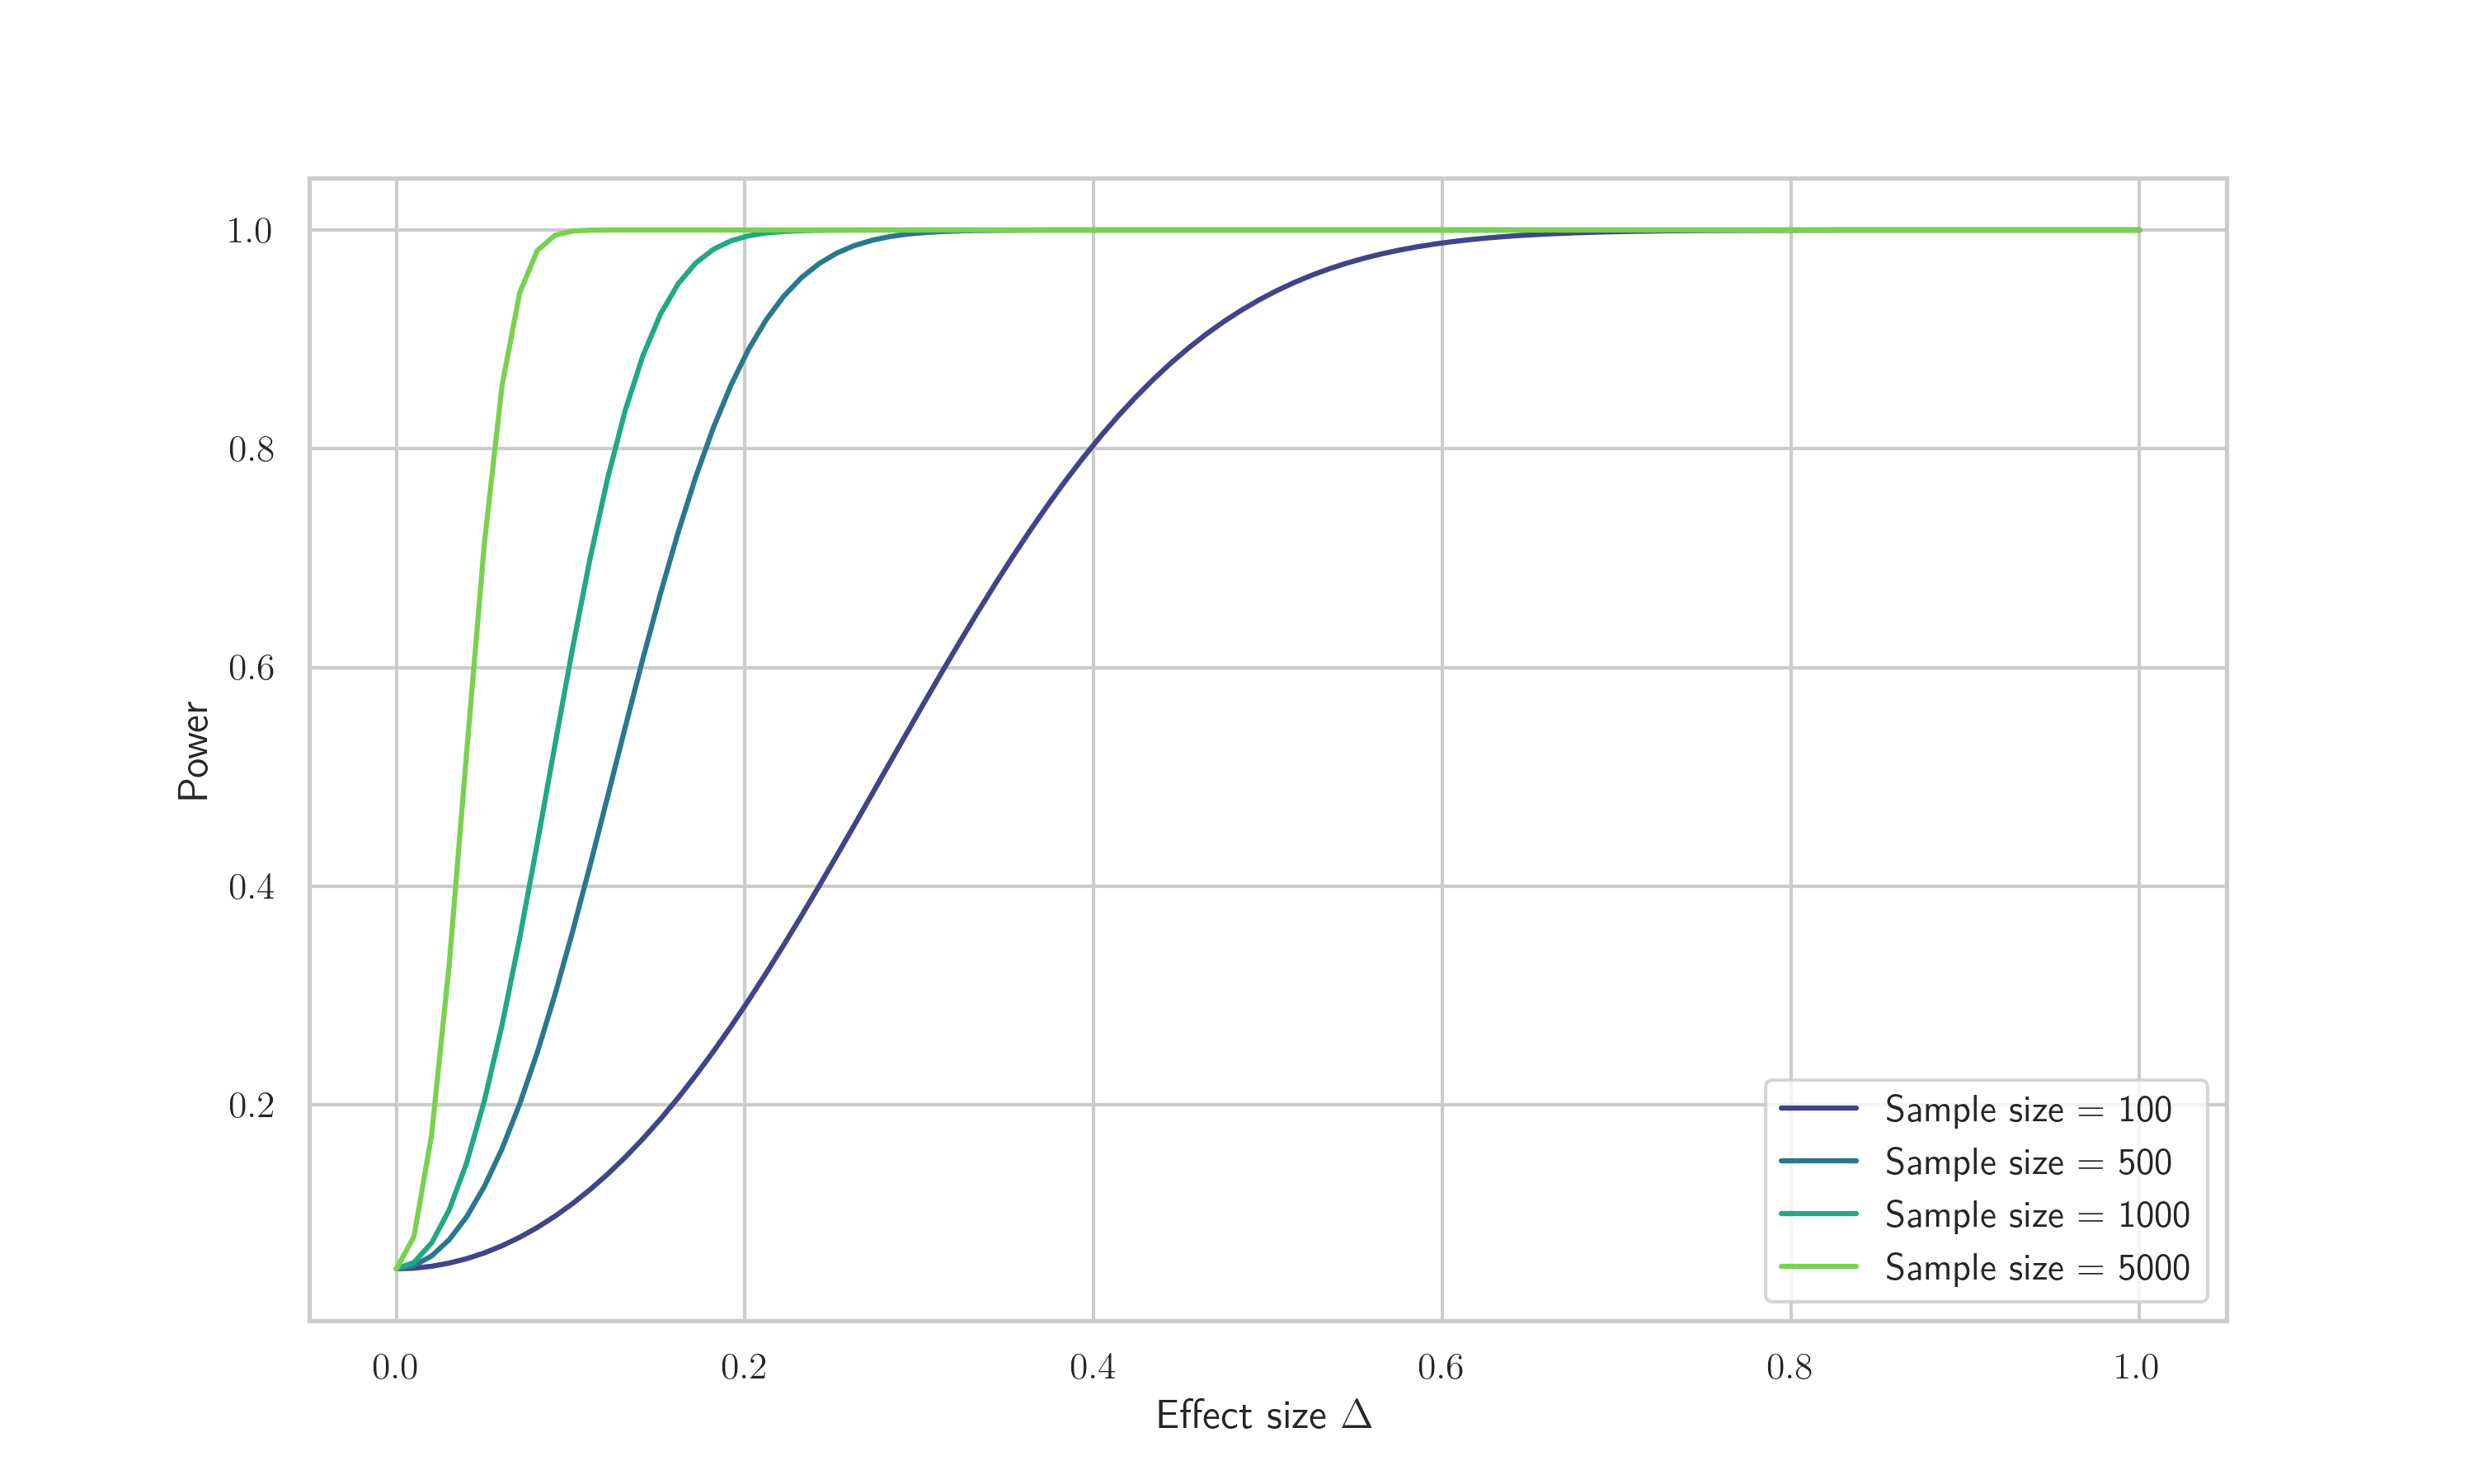
\includegraphics[width=\textwidth]{images/power_curve.png}
	\caption{Power curve for a two-sample t-test at a significance level of $\alpha = 0.05$. The~curve illustrates the relationship between the effect size $\Delta$ and the power of the test for various sample sizes.}
	\label{fig:power_curve}
\end{figure}
Figure~\ref{fig:power_curve} illustrates the power curve, demonstrating how the power of the test increases with larger effect sizes and sample sizes. This curve highlights the importance of designing an A/B test with sufficient power to detect true differences while minimizing the risk of~Type~I and Type~II~errors.

\myparagraph{Extensions and Variations in A/B Testing}

While classical A/B testing is robust, it can be extended and adapted to address more complex scenarios. For example, A/B/n testing involves comparing more than two variants simultaneously, which increases the risk of Type I errors due to multiple comparisons. This necessitates corrections such as the Bonferroni adjustment or controlling the False Discovery Rate (FDR) \cite{Benjamini1995, Holm1979}.

In situations where the assumptions of normality or homoscedasticity are violated, non-parametric tests like the Mann-Whitney U test or the Wilcoxon signed-rank test provide viable alternatives that do not rely on these assumptions \cite{Hollander2013}.

\subsection{Testing with Binary Random Variables}

A significant portion of A/B tests involves binary outcomes, such as whether a user clicks a button or makes a purchase. For such binary data, where outcomes follow a~ Bernoulli distribution, the classical t-test is not appropriate. Instead, alternative methods such as~the chi-square test and the Z-test for proportions are employed.

\myparagraph{Chi-Square Test for Two Independent Groups}

The chi-square test is used to determine whether there is a significant association between two categorical variables across two independent groups. In the context of A/B~testing, this typically involves comparing the success rates of two groups.

Given observed successes \( x_A \) and \( x_B \) in groups A and B, with total sample sizes \( n_A \)~and \( n_B \), the expected number of successes under the null hypothesis \( H_0 \) is:
\begin{equation*}
	E_A = \frac{(x_A + x_B)  n_A}{n_A + n_B}, \quad E_B = \frac{(x_A + x_B)  n_B}{n_A + n_B}.
\end{equation*}

The chi-square statistic is then calculated as:
\begin{equation*}
	\chi^2 = \frac{(x_A - E_A)^2}{E_A} + \frac{(x_B - E_B)^2}{E_B} + \frac{(n_A - x_A - (n_A - E_A))^2}{n_A - E_A} + \frac{(n_B - x_B - (n_B - E_B))^2}{n_B - E_B},
\end{equation*}
which follows a chi-square distribution with 1 degree of freedom under \( H_0 \) \cite{agresti2012}.

\myparagraph{Z-Test for Proportions}

When comparing the success proportions between two groups, a Z-test for proportions is often employed. The test statistic is calculated as:
\begin{equation}\label{eqn:Z_statistic}
	Z = \frac{\hat{p}_A - \hat{p}_B}{\sqrt{\hat{p}(1-\hat{p})\left(\frac{1}{n_A} + \frac{1}{n_B}\right)}},
\end{equation}
where \( \hat{p}_A \) and \( \hat{p}_B \) are the observed proportions of successes, and \( \hat{p} \) is the pooled proportion:

\[
\hat{p} = \frac{x_A + x_B}{n_A + n_B},
\]
with \( x_A \) and \( x_B \) being the number of successes in groups A and B \cite{Newcombe1998}.
\subsection{Practical Considerations}

Implementing A/B testing in practical settings requires addressing several key challenges to ensure the validity and reliability of the results. One critical factor is the proper randomization of participants. Randomization is essential for reducing bias, as it ensures that each participant has an equal probability of being assigned to either the control or~treatment group. This process helps balance confounding variables across groups, thereby preventing systematic differences that could skew the interpretation of the treatment effect \cite{Kohavi2013}.

Another crucial aspect is determining the appropriate sample size. The power of~a~statistical test, which is the probability of correctly rejecting a false null hypothesis, depends on the sample size, the effect size \( \Delta \), and the variance \( \sigma^2 \). For continuous outcomes, particularly those following a normal distribution, the required sample size to achieve a~desired power \( 1-\beta \) at a~specified significance level \( \alpha \) is given by:

\begin{equation*}
	n = \frac{2\sigma^2(Z_{\alpha/2} + Z_\beta)^2}{\Delta^2},
\end{equation*}

where \( Z_{\alpha/2} \) and \( Z_\beta \) are critical values from the standard normal distribution corresponding to the significance level and desired power, respectively \cite{cohen2013}. Ensuring an adequate sample size is vital for the test's ability to detect meaningful differences, thereby minimizing the risks of Type I errors (false positives) and Type II errors (false negatives) \cite{sullivan2012}.

\subsubsection{Sample Size for Bernoulli Distributions}

In many A/B testing scenarios, particularly those involving binary outcomes (e.g.,~click-through rates, conversion rates), the data is modeled using a Bernoulli distribution. In~such cases, the sample size calculation must account for the nature of binary data. The required sample size \( n \) for a Bernoulli distribution, assuming equal sample sizes in both groups, can be expressed in the following lemma:

\begin{lemma}[Sample Size for Bernoulli Distributions]\label{lem:sample_size}
	Let \( p_A \) and \( p_B \) represent the success probabilities of the control and treatment groups in a Bernoulli-distributed A/B~test. The~required sample size \( n \) for each group, assuming equal sample sizes, to achieve a~desired significance level \( \alpha \) and power \( 1-\beta \) is given by:
	\begin{equation}
		n = \frac{(p_A(1-p_A)+ p_B(1-p_B))(Z_{\alpha/2} + Z_\beta)^2}{(p_A - p_B)^2},
	\end{equation}
	where \( Z_{\alpha/2} \) and \( Z_\beta \) are the critical values corresponding to the significance level and power, respectively.
\end{lemma}
\noindent The proof of this lemma is provided in Appendix \ref{proof:sample_size}.

Lemma \ref{lem:sample_size} is particularly useful in designing A/B tests where the outcomes are binary, such as determining whether a user clicks a link or not. It ensures that the sample size is sufficient to detect a difference between the two proportions with the desired level of~confidence and power.

For instance, consider a scenario where the control group (A) has a conversion rate of 50\% ( \( p_A = 0.5 \) ), and the new feature being tested (B) is expected to decrease this rate to 45\% ( \( p_B = 0.45 \) ). Using the above formula, we can calculate the required sample size. Assuming a significance level \( \alpha = 0.05 \) and a power of \( 1-\beta = 0.95 \), with the critical values \( Z_{\alpha/2} \approx 1.96 \) and \( Z_\beta \approx 1.645 \), the necessary sample size \( n \) is approximately 2,593 for each group.

Understanding and accurately calculating the required sample size is crucial to the success of an A/B test, especially when dealing with binary outcomes. An underpowered study may fail to detect significant differences, leading to incorrect conclusions, while an~overpowered study may unnecessarily consume resources by requiring more participants than needed.

\section{Issues with Classical A/B Testing}

Classical A/B testing is a foundational methodology in experimental design, providing a straightforward approach to comparing two variants. However, despite its widespread use, classical A/B testing is not without its challenges. In real-world applications, various factors can compromise the validity and reliability of test results, particularly when the underlying assumptions of the classical approach do not hold. This section explores some of the most pressing issues associated with classical A/B testing, including the dangers of interim data analysis, the complications of multiple comparisons, and the impact of~external, time-varying influences.

\subsection{Peeking and Its Consequences}

A common pitfall in classical A/B testing is the practice of "peeking"—examining the data before the experiment is complete. In dynamic, fast-paced environments, the temptation to look at preliminary results can be strong, especially when decisions need to~be made quickly. However, peeking can severely undermine the statistical integrity of~an~A/B~test by inflating the Type I error rate, leading to an increased likelihood of~falsely detecting a difference when none exists.

The impact of peeking can be understood mathematically. Suppose an experimenter performs \( k \) interim analyses during an experiment, each at a significance level \( \alpha \). The~overall probability of making at least one Type I error is approximately:
\[
\alpha_{\text{overall}} \approx 1 - (1 - \alpha)^k.
\]
For instance, with \( \alpha = 0.05 \) and \( k = 5 \), the cumulative Type I error rate rises to about 0.226, meaning there is a 22.6\% chance of incorrectly rejecting the null hypothesis at least once during the experiment.

To mitigate the risks associated with peeking, several strategies can be employed:
\begin{itemize}
	\item \textbf{Fixed-Horizon Testing}: One straightforward approach is to predefine the sample size or duration of the experiment and refrain from examining the data until the experiment has concluded. This prevents premature decision-making based on~incomplete data.
	\item \textbf{Group Sequential Designs}: These designs allow for interim analyses at predetermined points while controlling the overall Type I error rate. Group sequential methods use stopping boundaries to determine whether the experiment should be~stopped early for efficacy, futility, or continued \cite{Pocock1977}.
	\item \textbf{Alpha Spending Functions}: This approach involves distributing the overall significance level \( \alpha \) across multiple analyses, maintaining the desired error rate while allowing flexibility in the timing of interim looks at the data \cite{DeMets1994}.
\end{itemize}

\subsection{Multiple Comparisons and False Discoveries}

Another significant challenge in classical A/B testing arises when multiple hypotheses are tested simultaneously or in rapid succession. This is particularly common in large-scale experiments where multiple variants or metrics are evaluated concurrently. The issue with multiple comparisons is that the risk of encountering a Type I error increases with each additional test.

To quantify this, consider a scenario where \( m \) independent hypotheses are tested, each at a significance level \( \alpha \). The probability of making at least one Type I error among these tests can be controlled by adjusting the significance level for each test using the Bonferroni correction:
\[
\alpha^* = \frac{\alpha}{m}.
\]
While effective in controlling the family-wise error rate (FWER), the Bonferroni correction can be overly conservative, especially when \( m \) is large, potentially leading to a loss of~statistical power \cite{Holm1979}.

To strike a better balance, the False Discovery Rate (FDR) control, introduced by~Benjamini and Hochberg, provides an alternative that is less conservative than the Bonferroni correction. FDR focuses on controlling the expected proportion of false positives among the rejected hypotheses, rather than merely preventing any Type I errors. The Benjamini-Hochberg procedure determines the threshold for significance by ordering the \( p \)-values and setting a cutoff where:
\[
p_{(k)} \leq \frac{k}{m} \alpha,
\]
where \( p_{(k)} \) is the \( k \)-th smallest \( p \)-value. This approach allows for more discoveries while keeping the false positive rate under control \cite{Benjamini1995}.

In more complex experimental setups, particularly those requiring multiple analyses over time, group sequential methods can be adapted to control the cumulative Type~I~error rate. These methods are valuable when tests are conducted sequentially, as they provide a~structured framework for managing the risk of Type I errors across multiple analyses~\cite{Pocock1977}.

\section{Game Theory and Decision Functions}

This section introduces the foundational concepts of game theory and decision functions, both of which are essential for understanding and optimizing A/B testing. We will first delve into game theory, exploring how strategic interactions between decision-makers can influence experimental outcomes, followed by a detailed discussion on decision functions in~statistical decision theory.


\subsection{Game Theory}

Game theory is the study of strategic interactions among rational decision-makers, where the outcome for each participant depends not only on their own actions but also on the actions of others. This framework is crucial for analyzing scenarios where multiple stakeholders or users interact in a shared environment, such as in A/B testing. By applying game-theoretic concepts, we can better understand and predict the behavior of different actors involved in the experiment, leading to more informed decisions and optimal outcomes.

\subsubsection{Fundamental Concepts in Game Theory}

Game theory is built on several foundational concepts, each essential for analyzing strategic interactions in A/B testing:

\begin{definition}[Players]
	In game theory, the decision-makers involved in the interaction are referred to as \textbf{players}. Each player aims to maximize their payoff, which depends on~the strategies chosen by all players. 
\end{definition}
\noindent
In the context of A/B testing, players can represent different teams within an organization (e.g., marketing, product development) or the users interacting with the variants being tested. Each player’s decision impacts not only their own outcome but also the outcomes of others, making the interplay of strategies critical.

\begin{definition}[Strategies]
	A \textbf{strategy} is a complete plan of action that a player follows throughout the game. The set of all possible strategies available to a player is known as~the \textbf{strategy space}.
\end{definition}
\noindent
In A/B testing, strategies might include decisions on sample size, timing of interim analyses, stopping criteria, or even how users interact with different variants. Each player’s strategy is formulated by anticipating the actions of others and choosing the course of action that maximizes their expected payoff.

\begin{definition}[Payoffs]
	The \textbf{payoff} is the reward or outcome that a player receives based on the combination of strategies chosen by all players. The payoff function \( u_i(s_1, s_2, \dots, s_n) \) assigns a numerical value to the outcome for player \( i \) given the strategy profile \( (s_1, s_2, \dots, s_n) \). 
\end{definition}
\noindent
In A/B testing, payoffs could be metrics such as conversion rates, revenue, or user engagement. The structure of the payoff function reflects the preferences of each player and the trade-offs involved in different strategic choices.

\begin{definition}[Games in Strategic Form]
	A game in \textbf{strategic form} (or normal form) is defined by:
	\begin{itemize}
		\item The set of players \( N = \{1, 2, \dots, n\} \).
		\item The strategy space \( S_i \) for each player \( i \).
		\item The payoff function \( u_i: S_1 \times S_2 \times \dots \times S_n \rightarrow \mathbb{R} \) for each player \( i \).
	\end{itemize}
\end{definition}
\noindent
The strategic form provides a snapshot of the game, capturing all possible strategies and their associated payoffs. This form is particularly useful for analyzing simultaneous-move games where players choose their strategies without knowledge of others' choices.
\begin{definition}[Nash Equilibrium]
	A \textbf{Nash equilibrium} is a strategy profile\\\( (s_1^*, s_2^*, \dots, s_n^*) \) where no player can improve their payoff by unilaterally changing their strategy:
	\[
	u_i(s_1^*, s_2^*, \dots, s_i^*, \dots, s_n^*) \geq u_i(s_1^*, s_2^*, \dots, s_i, \dots, s_n^*),
	\]
	for all \( i \) and for all alternative strategies \( s_i \).
\end{definition}
\noindent
The Nash equilibrium represents a stable outcome where each player’s strategy is the best response to the strategies of the other players \cite{nash1950non}. In A/B testing, reaching a Nash equilibrium implies that no team or user can improve their outcome by deviating from their current strategy, given the strategies of~others.

\subsubsection{Types of Games and Their Application to A/B Testing}

Game theory encompasses various types of games, each offering unique insights into A/B testing scenarios:

\myparagraph{Cooperative vs. Non-Cooperative Games}

In \textbf{cooperative games}, players can form binding agreements and collaborate to~achieve better outcomes. Cooperation allows players to pool their strategies and resources to~maximize collective payoffs. Conversely, \textbf{non-cooperative games} focus on strategic interactions where each player acts independently to maximize their payoff without binding agreements. Most A/B testing scenarios are modeled as non-cooperative games, where different teams or users act independently, pursuing their objectives.

\myparagraph{Static vs. Dynamic Games}

In \textbf{static games}, all players choose their strategies simultaneously, with no knowledge of~the other players' choices. These games capture scenarios where decisions are made without the ability to observe others' actions. In contrast, \textbf{dynamic games} involve sequential decision-making, where some players can observe earlier actions of others before making their choices. Dynamic games are particularly relevant in A/B testing when decisions are made in stages, such as during interim analyses or when adapting the experiment based on preliminary results.

\myparagraph{Complete vs. Incomplete Information Games}

In games of \textbf{complete information}, all players are fully informed about the payoff functions and strategies available to all other players. In contrast, \textbf{incomplete information games} involve scenarios where players have private information, such as their payoff function or the probability distribution of other players' payoffs. Incomplete information games are common in A/B testing, where different stakeholders may have private information about user preferences or the expected impact of the variants. \textbf{Bayesian games} are a specific type of incomplete information game where players have beliefs about the types of other players, represented by probability distributions \cite{Harsanyi1967}.

\subsubsection{Game Theory Applied to A/B Testing}

Several advanced game-theoretic concepts are particularly relevant to the analysis and design of A/B testing:

\begin{definition}[Mixed Strategy]
	A \textbf{mixed strategy} is a probability distribution over a~player's pure strategies. Rather than choosing a single strategy with certainty, a player randomizes over available strategies according to~specific probabilities. A \textbf{mixed strategy Nash equilibrium} occurs when each player's mixed strategy is the best response to~the mixed strategies of the other players. In A/B testing, mixed strategies could involve deploying variants probabilistically rather than deterministically, balancing exploration and exploitation in uncertain environments \cite{Aumann1974}.
\end{definition}

\begin{definition}[Correlated Equilibrium]
	A \textbf{correlated equilibrium} is a generalization of the Nash equilibrium, where players may coordinate their strategies based on signals from a correlation device. This concept allows for more flexible strategic interactions and can lead to outcomes where all players achieve higher payoffs compared to a Nash equilibrium. Correlated equilibria are relevant in A/B testing when an external signal or~trend (e.g., a seasonal effect or market shift) is observed by all stakeholders, allowing them to coordinate their strategies more effectively \cite{Aumann1987}.
\end{definition}

\begin{definition}[Repeated Games]
	\textbf{Repeated games} involve the same players playing a game multiple times. The strategies in repeated games can depend on the history of play, allowing for more complex interactions, such as cooperation, punishment, and reputation-building. In A/B testing, repeated games can model situations where the same or similar tests are conducted multiple times, with decisions in one test influencing future tests. Understanding repeated games helps in analyzing how long-term strategies evolve and how cooperation or competition between teams might develop over time.
\end{definition}

\begin{definition}[Multi-Armed Bandit Problems]
	The \textbf{multi-armed bandit problem} is a classic problem in game theory involving the allocation of resources among competing options (or "arms") to maximize cumulative rewards. In A/B testing, this translates to~dynamically allocating users to different variants based on their performance. The~challenge lies in balancing exploration (gathering information about the effectiveness of each variant) with exploitation (using the best-known variant to maximize rewards). Solutions such as \textbf{Thompson Sampling} and the \textbf{Upper Confidence Bound (UCB)} algorithm are commonly used in adaptive A/B testing to optimize the allocation of traffic among variants~\cite{Lai1985}.
\end{definition}

\subsubsection{Application of Game Theory to Real-World A/B Testing Scenarios}

Game theory provides valuable insights into several practical aspects of A/B testing:

\myparagraph{Stakeholder Interaction and Conflict Resolution}

In A/B testing, different teams within an organization often have conflicting objectives. For example, the marketing team may prioritize metrics that reflect short-term engagement, while the product development team might focus on long-term user retention. Game theory can model these interactions, helping to identify strategies that lead to a Nash equilibrium where all stakeholders are satisfied with the outcome. Additionally, game theory can be~used to design mechanisms that incentivize cooperation between teams, ensuring that the chosen variant balances the interests of all parties.

\myparagraph{User Behavior and Strategic Interaction}

Users in an A/B test are not passive participants; their behavior can influence the outcome of the test. For instance, users might adapt to changes in the user interface, or~their behavior might change based on their perceptions of the different variants. Game~theory provides a framework for anticipating such strategic behavior and designing tests that account for these interactions.

By modeling the users as players in a game, experimenters can predict how different test designs might influence user behavior and adjust their strategies accordingly. This~approach is particularly important in online experiments, where user behavior can have a significant impact on the validity of the test results.

\myparagraph{Dynamic and Adaptive Testing Strategies}

Game theory is also applicable in the design of dynamic and adaptive A/B testing strategies. For example, in a dynamic game, the experimenters might decide whether to~continue the test, stop it early, or switch to a different variant based on the data collected so far. This decision-making process can be modeled as a sequential game, where each stage of the test represents a move in the game.

%\subsection{Conclusion}
%%TODO to delate
%Game theory offers a rich and powerful framework for analyzing the strategic interactions that occur in A/B testing. By modeling the decisions of different stakeholders and users as a game, experimenters can gain deeper insights into how these interactions influence the outcome of the test. Game theory not only helps in identifying optimal strategies and equilibria but also provides a foundation for designing tests that are robust to strategic behavior and capable of balancing competing objectives.
%
%In the context of A/B testing, game theory enhances our understanding of how to~navigate complex decision-making environments, anticipate user behavior, and design experiments that lead to reliable and actionable results. As A/B testing continues to~evolve, the application of game theory will become increasingly important in ensuring that tests are both scientifically rigorous and strategically sound.
%


\subsection{Decision Functions in Statistical Decision Theory}

Statistical decision theory provides a framework for making optimal decisions under uncertainty. A decision function is central to this framework, as it maps observed data to~6actions in a way that seeks to minimize losses or maximize gains. This subsection delves into the core concepts, criteria for optimal decision-making, and examples of decision functions, particularly in the context of A/B testing.

\subsubsection{Basic Definitions and Concepts}

In any decision-making scenario, the true state of nature is denoted by a parameter \( \theta \in \Theta \), where \( \Theta \) is the parameter space. The decision-maker observes data \( X \in \mathcal{X} \) from the sample space \( \mathcal{X} \) and must choose an action \( a \in \mathcal{A} \), with \( \mathcal{A} \) being the action space.

\begin{definition}[Decision Function]
	A \textbf{decision function} \( \delta: \mathcal{X} \rightarrow \mathcal{A} \) is a rule that prescribes an action based on the observed data \( X \).
\end{definition}

The objective of a decision function is to guide the decision-making process in a way that optimizes outcomes under the uncertainty surrounding the true state of nature \( \theta \).

\begin{definition}[Loss Function]
	The quality of a decision is assessed using a \textbf{loss~function} \( L(\theta, a) \), which quantifies the cost associated with choosing action \( a \) when the true state is \( \theta \).
\end{definition}

The loss function plays a pivotal role in decision theory, as it encapsulates the consequences of different decisions under various scenarios.

\begin{definition}[Risk Function]
	The \textbf{risk function} \( R(\theta, \delta) \) represents the expected loss associated with the decision function \( \delta \) for a given parameter \( \theta \):
	\[
	R(\theta, \delta) = \mathbb{E}_{X \mid \theta}[L(\theta, \delta(X))] = \int_{\mathcal{X}} L(\theta, \delta(x)) \, p(x \mid \theta) \, dx,
	\]
	where \( p(x \mid \theta) \) is the probability density function of \( X \) given \( \theta \).
\end{definition}

The risk function provides a comprehensive measure of how well a decision function performs across different possible states of nature.

\subsubsection{Optimality Criteria in Decision Functions}

Different criteria are employed to evaluate and select decision functions, each reflecting a distinct approach to managing risk and uncertainty:

\begin{definition}[Bayes Criterion]
	The \textbf{Bayes criterion} integrates prior knowledge about the parameter \( \theta \) through a prior distribution \( \pi(\theta) \). The Bayes risk is the expected value of the risk function over this prior:
	\[
	r(\pi, \delta) = \int_{\Theta} R(\theta, \delta) \, \pi(\theta) \, d\theta.
	\]
\end{definition}

\begin{definition}[Bayes Decision Function]
	The decision function \( \delta^* \) that minimizes the Bayes risk is known as the \textbf{Bayes decision function}:
	\[
	\delta^*(x) = \arg \min_{a \in \mathcal{A}} \int_{\Theta} L(\theta, a) \, \pi(\theta \mid x) \, d\theta,
	\]
	where \( \pi(\theta \mid x) \) is the posterior distribution of \( \theta \) given the observed data \( x \).
\end{definition}

The Bayes criterion is especially useful when prior information about \( \theta \) is reliable, allowing the decision-maker to combine prior knowledge with observed data to make well-informed decisions \cite{Berger1985}.

\begin{definition}[Minimax Criterion]
	The \textbf{minimax criterion} is a conservative approach that focuses on minimizing the maximum possible risk:
	\[
	\delta^* = \arg \min_{\delta} \max_{\theta \in \Theta} R(\theta, \delta).
	\]
\end{definition}

This criterion is particularly relevant in scenarios with high uncertainty or severe consequences for incorrect decisions, as it ensures robustness against the worst-case scenario \cite{wald1949statistical}.

\begin{definition}[Admissibility and Dominance]
	A decision function \( \delta \) is considered \textbf{admissible} if no other decision function \( \delta' \) exists that dominates it. Specifically:
	\[
	R(\theta, \delta') \leq R(\theta, \delta) \quad \text{for all } \theta \in \Theta,
	\]
	with strict inequality for some \( \theta_0 \in \Theta \).
\end{definition}

Admissibility ensures that a decision function is not universally inferior, making it~a~candidate for optimality under various criteria. An admissible decision function is~robust across different scenarios, ensuring that it performs well in uncertain environments \cite{lehmann2006theory}.

\begin{definition}[Pareto Optimality]
	In multi-objective decision-making, \textbf{Pareto optimality} evaluates decision functions based on multiple criteria. A decision function \( \delta \)~is~Pareto optimal if no other function \( \delta' \) improves one objective without worsening another:
	\[
	R_i(\theta, \delta') \leq R_i(\theta, \delta) \quad \text{for all } i,
	\]
	with strict inequality for at least one \( i \).
\end{definition}

Pareto optimality is especially relevant in A/B testing when balancing the interests of~different stakeholders, ensuring a trade-off that satisfies multiple objectives \cite{Miettinen1999}.

\subsubsection{Examples of Decision Functions in A/B Testing}

In A/B testing, decision functions guide whether to adopt a new variant (B) over a~control (A) based on observed data. Common decision functions include:

\begin{example}[Threshold-Based Decision Function]
	A simple decision function is~to~reject the null hypothesis \( H_0 \) if the test statistic \( T(X) \) exceeds a critical value \( c \):
	\[
	\delta(X) = 
	\begin{cases} 
		\text{Adopt B} & \text{if } T(X) > c, \\
		\text{Retain A} & \text{otherwise}.
	\end{cases}
	\]
\end{example}

This function reflects a decision rule where the loss function accounts for the costs of~adopting a suboptimal variant, and the risk function quantifies the expected losses due to Type I and Type II errors.

\begin{example}[Bayesian Decision Function]
	In a Bayesian framework, the decision to~adopt variant B over A depends on the posterior probability that B is better than A:
	\[
	\delta(X) = 
	\begin{cases} 
		\text{Adopt B} & \text{if } \pi(\theta_B > \theta_A \mid X) > \gamma, \\
		\text{Retain A} & \text{otherwise}.
	\end{cases}
	\]
\end{example}

The threshold \( \gamma \) reflects the decision-maker’s tolerance for risk, with higher values indicating a more conservative approach. This decision function is informed by both prior beliefs and current evidence.

\begin{example}[Sequential Decision Function]
	In sequential A/B testing, the decision function involves continuous monitoring and stopping the test once sufficient evidence is~gathered:
	\[
	\delta(X) = 
	\begin{cases} 
		\text{Stop and adopt B} & \text{if } T_n > c, \\
		\text{Stop and retain A} & \text{if } T_n < -c, \\
		\text{Continue testing} & \text{otherwise}.
	\end{cases}
	\]
\end{example}

Sequential decision functions are effective in reducing sample sizes by allowing early stopping when there is strong evidence favoring one variant over the other \cite{wald2004sequential}.

\subsubsection{Decision Functions in the Context of Loss Functions}

The choice of a decision function is closely linked to the choice of a loss function, as~different loss functions lead to different optimal decision rules. Common loss functions include:

\begin{example}[Binary Loss Function]
	The \textbf{binary loss function} assigns a loss of 0 for a correct decision and 1 for an incorrect decision:
	\[
	L(\theta, a) = 
	\begin{cases} 
		0 & \text{if the correct decision is made}, \\
		1 & \text{if the incorrect decision is made}.
	\end{cases}
	\]
\end{example}

This loss function is common in hypothesis testing, where the goal is to minimize the probability of making an incorrect decision.

\begin{example}[Quadratic Loss Function]
	The \textbf{quadratic loss function} penalizes errors based on the square of the difference between the estimated and true parameter values:
	\[
	L(\theta, a) = (\theta - a)^2.
	\]
\end{example}

This function is often used in estimation problems, encouraging decisions that minimize the mean squared error.

\begin{example}[Asymmetric Loss Function]
	In some cases, the cost of different types of~errors is not symmetric. For instance, in A/B testing, the cost of adopting a suboptimal variant might be higher than the cost of missing a small improvement. An \textbf{asymmetric loss function} reflects this by assigning different penalties to different types of errors:
	\[
	L(\theta, a) = 
	\begin{cases} 
		\lambda_1(\theta - a) & \text{if } \theta > a, \\
		\lambda_2(a - \theta) & \text{if } \theta \leq a,
	\end{cases}
	\]
	where \( \lambda_1 \) and \( \lambda_2 \) are different penalty coefficients.
\end{example}

This type of loss function can lead to decision functions that are more conservative or~aggressive, depending on the relative costs of the errors.
%\subsection{Conclusion}
%TODO conclusion
%Decision functions are fundamental to the application of statistical decision theory in A/B testing. They provide a structured approach to making optimal decisions based on observed data, balancing different objectives and uncertainties. By formalizing the decision-making process through decision functions, experimenters can ensure that their choices are statistically justified and aligned with the overall goals of the test.
%
%In A/B testing, decision functions are essential for determining when to stop the test, which variant to adopt, and how to balance competing interests and uncertainties. The~choice of an appropriate decision function depends on the specific context of the test, including the available prior information, the nature of the loss function, and the desired balance between different types of errors.


\section{Sequential A/B Testing Methods}

Sequential A/B testing represents an advanced methodology that enhances traditional A/B testing by allowing for continuous data evaluation and adaptive decision-making. Unlike classical A/B testing, which relies on a fixed sample size and makes decisions only after all data is collected, sequential A/B testing evaluates data as it is accumulated. This approach can lead to earlier conclusions, more efficient use of resources, and ethical advantages, particularly in situations where prolonged exposure to inferior treatments or~variants is undesirable.

\subsection{Theoretical Foundations of Sequential A/B Testing}

Sequential A/B testing is grounded in the principles of sequential analysis, which permits hypothesis testing as data accumulates rather than requiring a fixed sample size. This method is~particularly advantageous in scenarios where early decision-making is~crucial, such as in online experiments or clinical trials, where rapid iteration or ethical considerations are paramount.

\subsubsection{Hypothesis Formulation}
As with traditional A/B testing, the first step in sequential A/B testing is to define the null and alternative hypotheses. The null hypothesis \( H_0 \) posits that there is no~difference in~the mean outcomes between the two variants, while the alternative hypothesis \( H_1 \)~suggests a difference:
\begin{align*}
	H_0 &: \mu_A = \mu_B, \\
	H_1 &: \mu_A \neq \mu_B.
\end{align*}
where \( \mu_A \) and \( \mu_B \) represent the expected values of the performance metric (such as~conversion rates) for the control (A) and treatment (B) groups, respectively. The objective of the sequential A/B test is to decide whether to accept \( H_0 \) or \( H_1 \) based on the data collected up to a certain point, with the flexibility to stop the test as soon as sufficient evidence is~gathered.

\subsubsection{Sequential Probability Ratio Test (SPRT)}

The Sequential Probability Ratio Test (SPRT), developed by Abraham Wald, is the cornerstone of sequential analysis and is widely applicable to A/B testing. SPRT provides a systematic method for continuously evaluating the evidence in favor of \( H_0 \) or \( H_1 \) as data is collected.

\myparagraph{Likelihood Ratio}

At each stage \( n \) of data collection, the likelihood ratio \( \Lambda_n \) is calculated as:

\[
\Lambda_n = \frac{\prod_{i=1}^{n} f(X_i; \theta_1)}{\prod_{i=1}^{n} f(X_i; \theta_0)},
\]

where \( f(X_i; \theta) \) is the probability density function (or probability mass function in~the case of discrete data) of the observation \( X_i \) under the parameter \( \theta \). For A/B testing, \( \theta_0 \)~and~\( \theta_1 \) represent the parameters under the null and alternative hypotheses, respectively.

Alternatively, the log-likelihood ratio \( \log \Lambda_n \) can be expressed as:

\[
\log \Lambda_n = \sum_{i=1}^{n} \log \left(\frac{f(X_i; \theta_1)}{f(X_i; \theta_0)}\right),
\]

which accumulates evidence for or against \( H_0 \) as data is observed. The decision at~stage \( n \) is then based on this accumulated evidence.

%\myparagraph{Decision Rule}
%
%The decision to continue, stop, or reject the null hypothesis in SPRT is based on~comparing the likelihood ratio \( \Lambda_n \) to two predefined thresholds \( A \) and \( B \), where \( A<B \):
%
%\begin{align*}
%	\text{If } \Lambda_n &\geq B, \quad \text{reject } H_0 \text{ in favor of } H_1, \\
%	\text{If } \Lambda_n &\leq A, \quad \text{accept } H_0 \text{ and stop the test}, \\
%	\text{If } A < \Lambda_n &< B, \quad \text{continue collecting data}.
%\end{align*}


%\myparagraph{Expected Sample Size}
%TODO to rm
%%TODO nie wiem czy nei usunąć
%The efficiency of the SPRT is reflected in its ability to minimize the expected sample size \( E(n) \). Under the assumptions of the test, the expected sample size required to reach a~decision is often significantly smaller than that required by a fixed-sample test with the same error rates. 
%
%\begin{theorem}
%The expected sample size \( E(n) \) can be approximated using Wald's approximation:
%\[
%E(n) \approx \frac{\log B - \log A}{I(\theta_0, \theta_1)},
%\]
%where \( I(\theta_0, \theta_1) \) is the Kullback-Leibler information number, defined as:
%
%\[
%I(\theta_0, \theta_1) = \mathbb{E}_{\theta_1}\left[\log \left(\frac{f(X; \theta_1)}{f(X; \theta_0)}\right)\right].
%\]
%\end{theorem}
%
%This information measure quantifies the expected log-likelihood ratio under the alternative hypothesis and directly influences the efficiency of the SPRT.

\subsubsection{Mixture Sequential Probability Ratio Test (mSPRT)}

The Mixture Sequential Probability Ratio Test (mSPRT) extends the classical SPRT to~handle cases where the alternative hypothesis is not a single point but a range of possible values. This approach is particularly useful in practical A/B testing scenarios where the effect size between the control and treatment groups is uncertain.

\myparagraph{Mixture Likelihood Ratio}

In mSPRT, instead of testing against a fixed alternative \( \theta_1 \), the test considers a mixture of possible alternatives \( \Theta_1 \). The likelihood ratio is then modified to integrate over this range:

\[
\Lambda_n = \frac{\int_{\Theta_1} w(\theta) \prod_{i=1}^{n} f(X_i; \theta) \, d\theta}{\prod_{i=1}^{n} f(X_i; \theta_0)},
\]

where \( w(\theta) \) is a weighting function that reflects prior beliefs about the distribution of~\( \theta \) within the space \( \Theta_1 \). This mixture approach allows the test to be more robust against uncertainty in the effect size, providing greater flexibility and adaptability in practical A/B testing applications.

\myparagraph{Decision Rule}

The decision-making process in mSPRT follows the same structure as in SPRT but applies to the mixture likelihood ratio \( \Lambda_n \):

\begin{align*}
	\text{If } \Lambda_n &\geq B, \quad \text{reject } H_0 \text{ in favor of } H_1, \\
	\text{If } \Lambda_n &\leq A, \quad \text{accept } H_0 \text{ and stop the test}, \\
	\text{If } A < \Lambda_n &< B, \quad \text{continue collecting data}.
\end{align*}
The thresholds \( A \) and \( B \) are chosen to control the Type I error rate \( \alpha \) and the Type~II~error rate \( \beta \):

\[
A = \frac{1 - \beta}{\alpha}, \quad B = \frac{\beta}{1 - \alpha}.
\]
These thresholds ensure that the test maintains the desired error rates while allowing for early stopping if sufficient evidence accumulates.


By considering a range of plausible effect sizes, mSPRT enhances the robustness of the decision-making process, particularly in environments where the effect size is uncertain or~variable.

\myparagraph{Bayesian Connection}

There is a natural connection between mSPRT and Bayesian methods, as the weighting function \( w(\theta) \) can be interpreted as a prior distribution over the parameter space \( \Theta_1 \). This Bayesian interpretation allows for a seamless integration of prior knowledge into the sequential testing framework, enhancing the flexibility and adaptability of the method.

%\myparagraph{Visualization: Likelihood Surface of mSPRT}
%
%%TODO nie wiem czy nie usunac
%A potential visualization could involve plotting the likelihood surface across the parameter space \( \Theta_1 \). This 3D plot or contour map would depict how the mixture likelihood ratio evolves as data accumulates, illustrating the test's ability to account for uncertainty in the effect size.

\subsubsection{Stopping Rules and Error Control}

A key feature of sequential A/B testing is the implementation of stopping rules, which determine when the test should conclude. The stopping rule \( \tau = \min\{n:\Lambda_n \le A \vee \Lambda_n \ge B\}\) is a random variable representing the time (or number of observations) at which the test stops. The stopping rule is crucial for controlling the overall error rates \( \alpha \) and \( \beta \), ensuring that the sequential nature of the test does not inflate these rates.
\myparagraph{Theoretical Foundations}

Consider a scenario where we have paired data \((x_i, y_i)\) for \(i = 1, 2, \dots, t\), where \(x_i\) and \(y_i\) represent the outcomes from two different populations or treatments (e.g., control and treatment groups in an A/B test). The goal is to test the hypothesis \(H: \theta_1 \leq \theta_2\), where \(\theta_1\)~and \(\theta_2\) are parameters of interest (e.g., means or proportions) for the two populations.

Girshick's test reformulates the SPRT for this paired data context by defining two specific hypotheses:
\begin{align*}
	H_0: &\quad \theta_1 = \theta_0^1 \quad \text{and} \quad \theta_2 = \theta_0^2, \\
	H_1: &\quad \theta_1 = \theta_0^2 \quad \text{and} \quad \theta_2 = \theta_0^1.
\end{align*}
where \(\theta_0^1\) and \(\theta_0^2\) represent specific values that define the magnitude of difference deemed important for business decisions.

\begin{example}[Normally Distributed Data with Equal Variances and Different Means]
	
	
	Consider the case where the observations \(x_i\) and \(y_i\) are normally distributed with the same variance \(\sigma^2\), but different means \(\mu_1 = \theta_1\) and \(\mu_2 = \theta_2\). The data can be modeled as:
	\begin{align*}
		x_i &\sim \mathcal{N}(\theta_1, \sigma^2), \\
		y_i &\sim \mathcal{N}(\theta_2, \sigma^2),
	\end{align*}
	where \(\mathcal{N}(\mu, \sigma^2)\) denotes a normal distribution with mean \(\mu\) and variance \(\sigma^2\).
	The probability ratio test statistic after \(t\) pairs of data is given by:
	\begin{align*}
		\frac{p_1^t}{p_0^t} &= \prod_{i=1}^{t} \frac{f_{\theta_0^2}(x_i) f_{\theta_0^1}(y_i)}{f_{\theta_0^1}(x_i) f_{\theta_0^2}(y_i)}.
	\end{align*}

	This can be simplified to:
	\begin{align}\label{eqn:normal_prts}
		\frac{p_1^t}{p_0^t} &= \exp\left(\frac{\theta_0^2 - \theta_0^1}{\sigma^2} \sum_{i=1}^{t} (x_i - y_i)\right).
	\end{align}
	The detailed proof of this simplification is provided in the appendix \ref{proof:normal_prts}.
	
	Taking the logarithm, the log-likelihood ratio becomes:
	\begin{align*}
		\log \left(\frac{p_1^t}{p_0^t}\right) &= \frac{\theta_0^2 - \theta_0^1}{\sigma^2}  \sum_{i=1}^{t} (x_i - y_i).
	\end{align*}
	
	This log-likelihood ratio can be used to make decisions at each stage of data collection, where the test will continue until the log-likelihood ratio exceeds a certain threshold, indicating sufficient evidence to reject the null hypothesis.
\end{example}

\begin{example}[Bernoulli Distributed Data with Different Success Probabilities]
	Consider the case where the outcomes \(x_i\) and \(y_i\) are Bernoulli distributed with success probabilities \(\theta_1 = p_1\) and \(\theta_2 = p_2\), respectively. The data can be modeled as:
	\begin{align*}
		x_i &\sim \text{Bernoulli}(\theta_1), \\
		y_i &\sim \text{Bernoulli}(\theta_2),
	\end{align*}
	where \(\text{Bernoulli}(p)\) denotes a Bernoulli distribution with success probability \(p\).
	
	The probability ratio test statistic after \(t\) pairs of data is given by:
	\begin{align*}
	\frac{p_1^t}{p_0^t} &= \prod_{i=1}^{t} \frac{f_{\theta_0^2}(x_i) f_{\theta_0^1}(y_i)}{f_{\theta_0^1}(x_i) f_{\theta_0^2}(y_i)}.
	\end{align*}

	This can be simplified to:
	\begin{align}\label{eqn:binomial_prts}
		\frac{p_1^t}{p_0^t} &= \left(\frac{\theta_0^2(1-\theta_0^1)}{\theta_0^1(1-\theta_0^2)}\right)^{\sum_{i=1}^{t} (x_i - y_i)}.
	\end{align}
	The detailed proof of this simplification is provided in the appendix \ref{proof:bernoulli_prts}.
	
	Taking the logarithm, the log-likelihood ratio becomes:
	\begin{align*}
		\log \left(\frac{p_1^t}{p_0^t}\right) &= \log \left(\frac{\theta_0^1(1-\theta_0^2)}{\theta_0^2(1-\theta_0^1)}\right)\sum_{i=1}^{t} (y_i - x_i).
	\end{align*}
	
	Again, this log-likelihood ratio is used to evaluate the evidence in favor of the alternative hypothesis \(H_1\) as data is collected.
\end{example}

\begin{definition}[Deviance Measure For Bernoulli Distribution]
	The deviance measure \(\nu(\theta_1, \theta_2)\) for Bernoulli distributions is given by:
	\begin{align*}
		\nu(\theta_1, \theta_2) &= \log \left(\frac{(1 - \theta_2)\theta_1}{(1 - \theta_1)\theta_2} \right).
	\end{align*}
\end{definition}

\begin{definition}[Deviance Measure For Normally Distribution]
	The deviance measure \(\nu(\theta_1, \theta_2)\) for normally distributed data with equal variances is given by:
	\begin{align*}
		\nu(\theta_1, \theta_2) &= \frac{\theta_2 - \theta_1}{\sigma^2}.
	\end{align*}
\end{definition}

This deviance measure has several important properties:
\begin{align*}
	\nu(\theta_1, \theta_2) &= 0 \quad \text{if } \theta_1 = \theta_2, \\
	\nu(\theta_1, \theta_2) &> 0 \quad \text{if } \theta_2 > \theta_1, \\
	\nu(\theta_1, \theta_2) &< 0 \quad \text{if } \theta_2 < \theta_1.
\end{align*}

These deviance measures can be used to divide the parameter space into distinct regions based on a threshold \(\delta > 0\), which informs the decision-making process in hypothesis testing.

\begin{align*}
	\omega_a &= \{\nu(p_1, p_2) < -\delta\}, \\
	\omega_r &= \{\nu(p_1, p_2) > \delta\}, \\
	\omega_o &= \{-\delta \leq \nu(p_1, p_2) \leq \delta\}.
\end{align*}

These regions correspond to:
\begin{itemize}
	\item \(\omega_a\): Acceptance region where \(H_0\) is preferred.
	\item \(\omega_r\): Rejection region where \(H_1\) is preferred.
	\item \(\omega_o\): Indifference region where neither hypothesis is strongly supported.
\end{itemize}

\begin{figure}[H]
	\centering
	\begin{subfigure}{.5\textwidth}
		\centering
		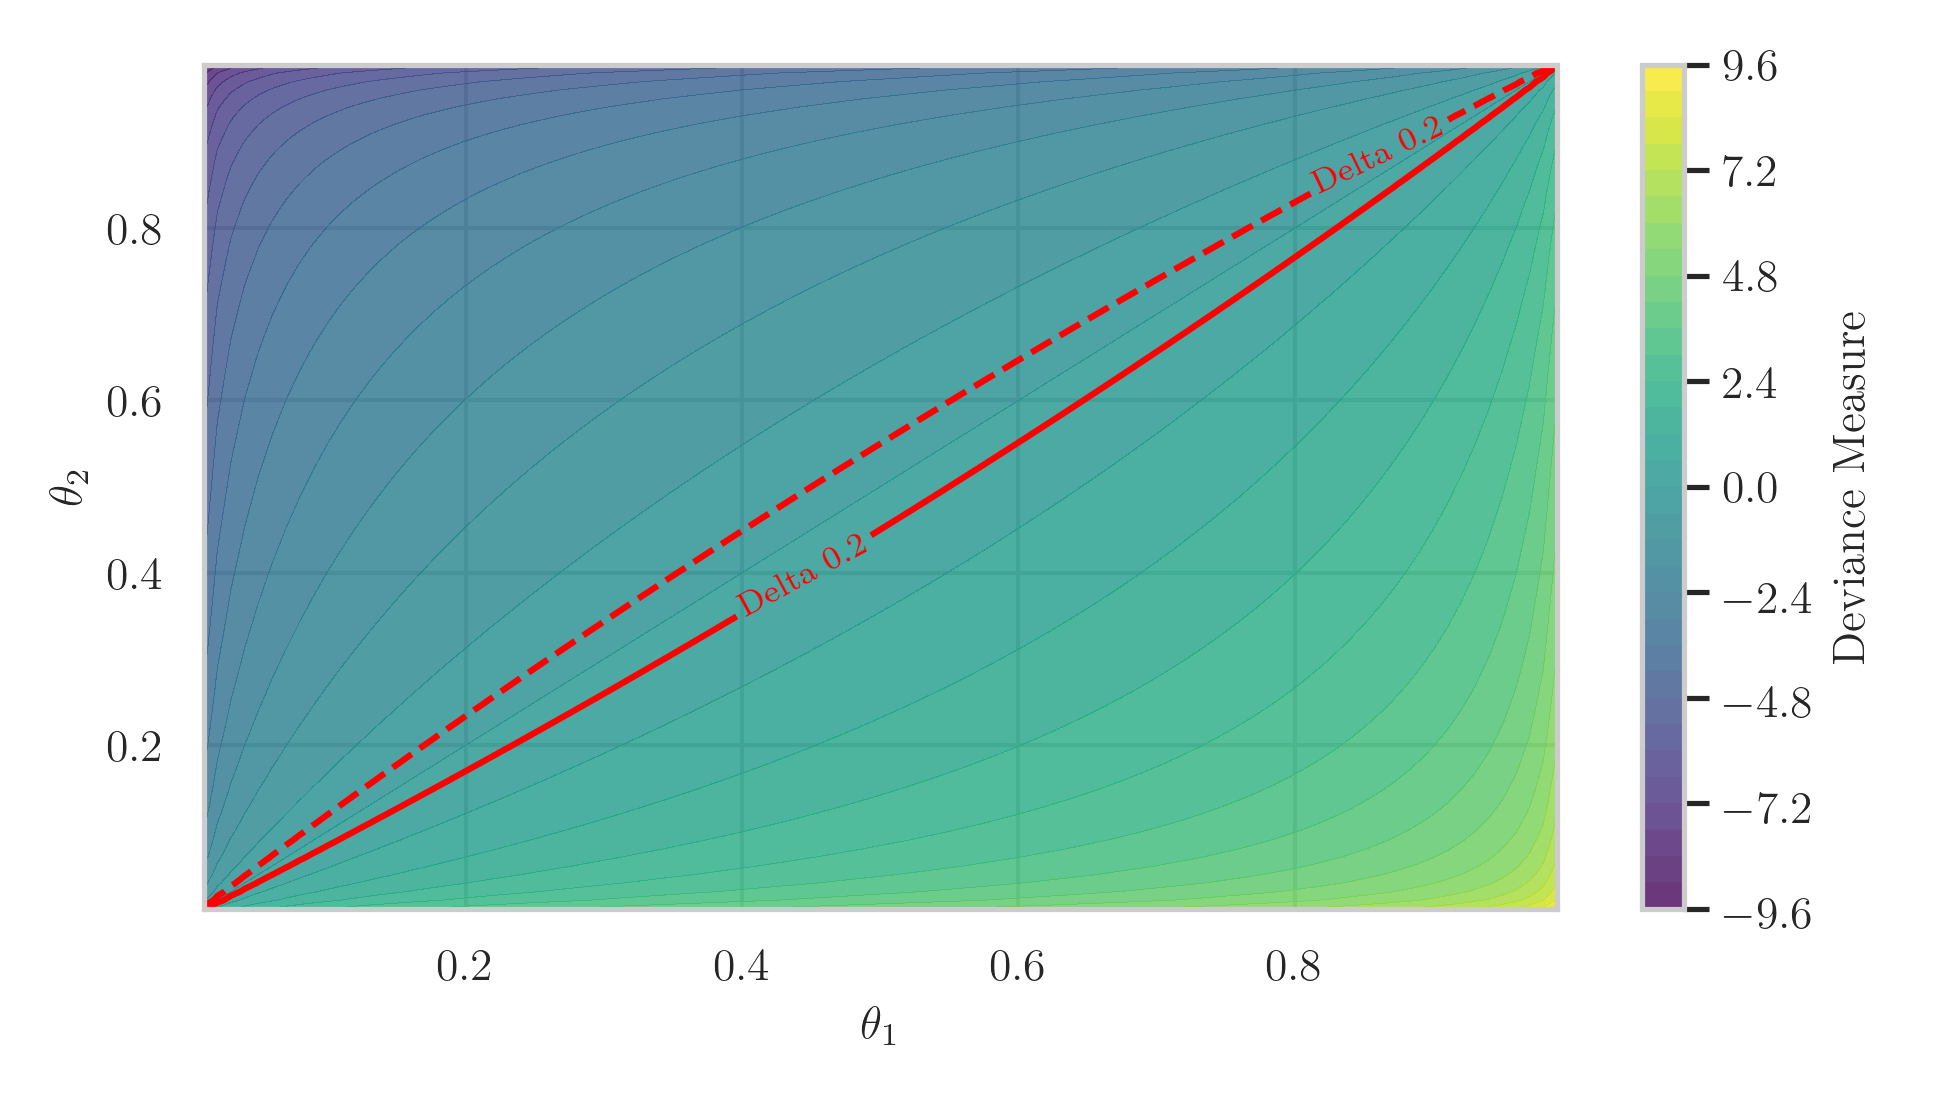
\includegraphics[width=1\linewidth]{images/bernoulli_deviance.png}
		\caption{Bernoulli distribution.}
		\label{fig:bernoulli_deviance}
	\end{subfigure}%
	\begin{subfigure}[r]{.5\textwidth}
		\centering
		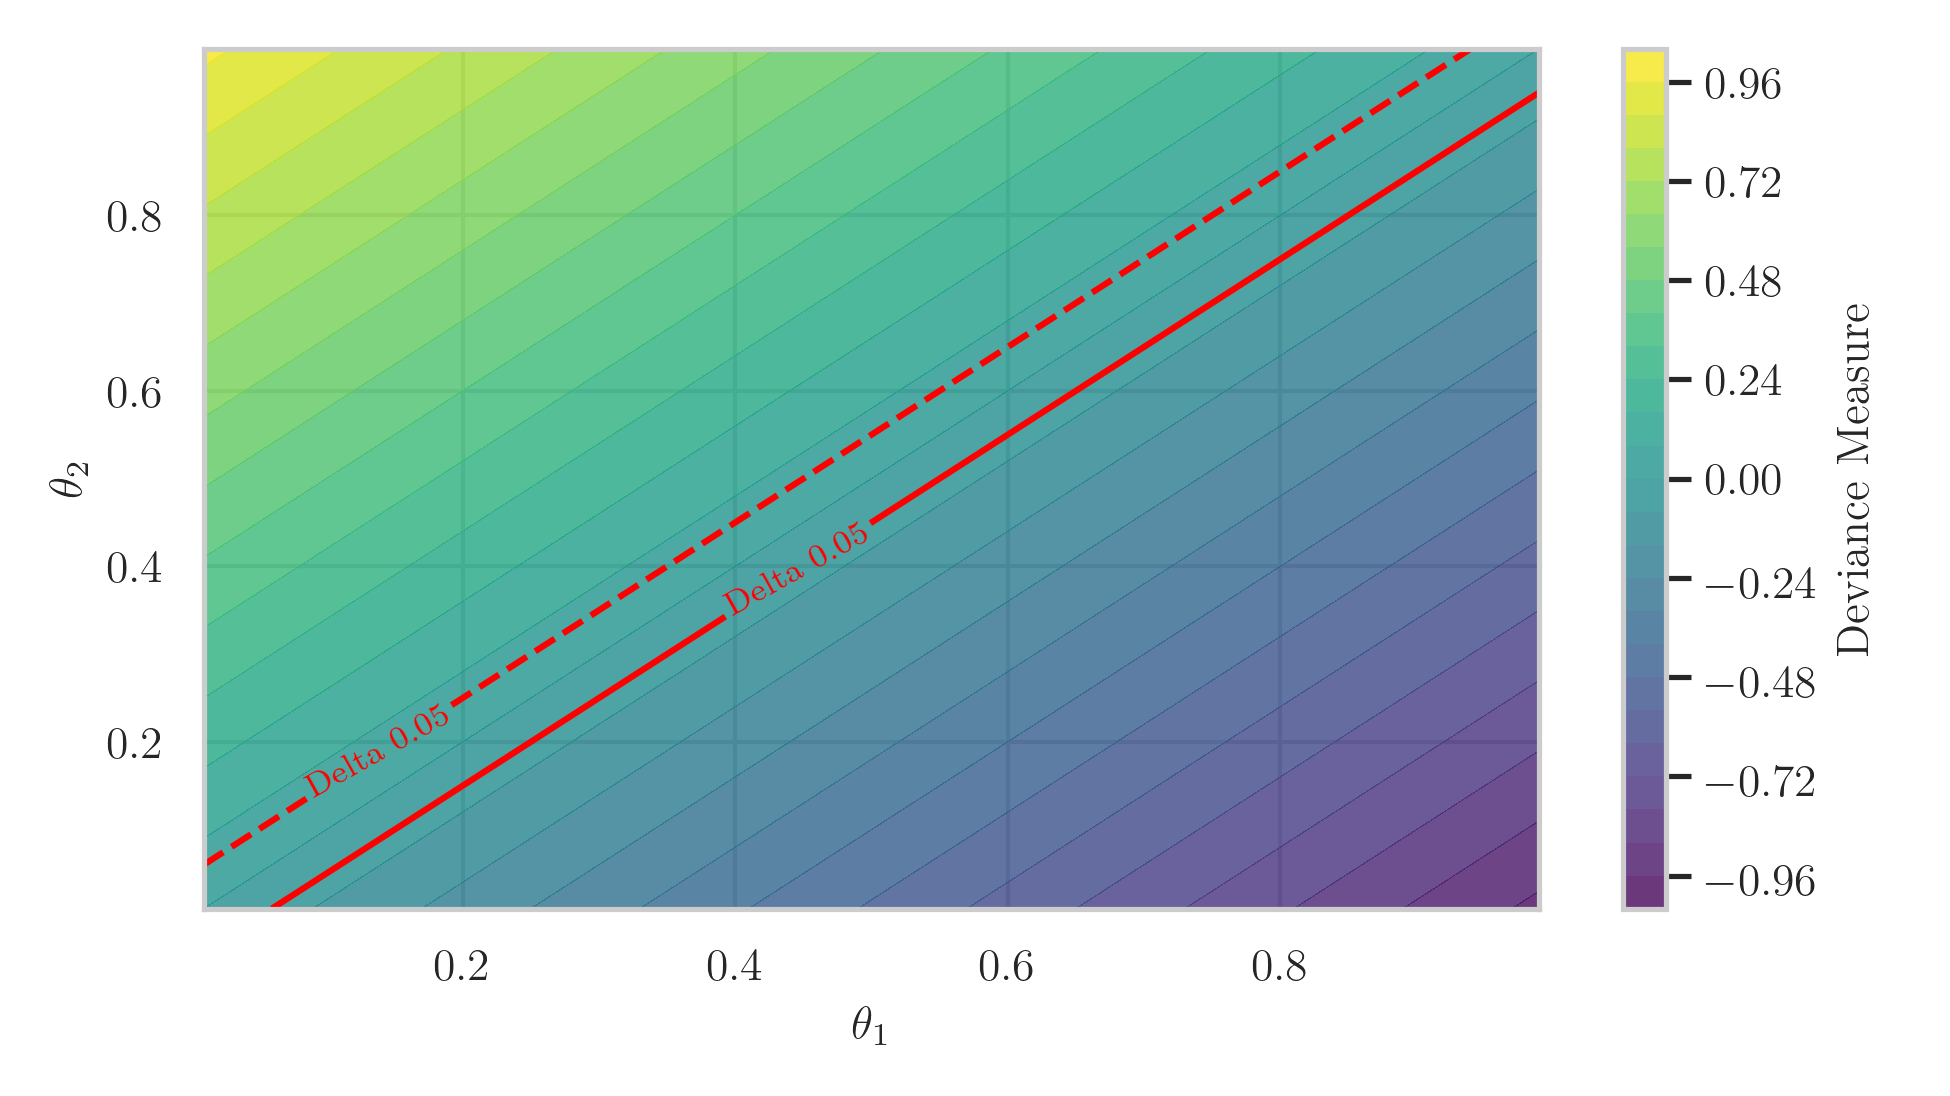
\includegraphics[width=1\linewidth]{images/normal_deviance.png}
		\caption{Normal distribution with unit Variance.}
		\label{fig:normal_deviance}
	\end{subfigure}
	\caption{Visualization of the deviance measure for different values of \(\delta\).}
	\label{fig:deviance}
\end{figure}

Figure \ref{fig:bernoulli_deviance} illustrates the deviance measure for the Bernoulli distribution with a~threshold of \(\delta = 0.2\).~The narrowing of the uncertainty boundaries is evident, reflecting a~decrease in the variance of the test statistic for the corresponding values of \(\theta_1\) and \(\theta_2\).~As \(\theta_1\) and \(\theta_2\)~diverge, the test gains increased confidence in rejecting the null hypothesis, indicating a~stronger evidence against \(H_0\).

Conversely, Figure \ref{fig:normal_deviance} demonstrates the deviance measure for the normal distribution with a threshold of \(\delta = 0.05\). Here, the boundaries are represented as linear functions, suggesting that the relationship between \(\theta_1\) and \(\theta_2\) in the normal distribution is more linear and predictable. The linearity simplifies the interpretation, as the change in deviance is~directly proportional to the difference between \(\theta_1\) and \(\theta_2\), providing a clear and consistent measure of deviation from the null hypothesis.


\myparagraph{Decision Rule}

Girshick’s double dichotomy test involves setting a threshold \(\delta > 0\) and continuously evaluating the log-likelihood ratio as new data is collected. At each time point \(t\), with \(t\)~pairs of observations, the log-likelihood ratio can be expressed as:
\[
Z_t = \log \left(\frac{p_1^t}{p_0^t}\right) = -\delta  t
 (\bar{Y}_t - \bar{X}_t).
\]

This expression demonstrates that the log probability ratio \(Z_t\) is a function of three factors: the risk tolerance \(\delta\), the total number of observations \(t\), and the difference between the average outcomes \((\bar{Y}_t - \bar{X}_t)\) of the two groups. This interpretation is central to~understanding the sequential Girshick test, as it shows how the cumulative evidence in favor of one hypothesis builds up based on the size of the sample and the observed difference between the two groups.

Using this formulation, the decision rule for Girshick’s test in the context of sequential A/B testing can be structured as follows. The data collection and analysis continue until the log-likelihood ratio \(Z_t\) reaches one of the predefined thresholds \(A\) or \(B\), which are determined by the desired error rates \(\alpha\) (Type I) and \(\beta\) (Type II):

\[
\text{If } Z_t \geq \log B, \text{ reject } H_0,
\]
\[
\text{If } Z_t \leq \log A, \text{ accept } H_0,
\]
\[
\text{If } \log A < Z_t < \log B, \text{ continue testing}.
\]

This decision rule ensures that testing proceeds until there is strong enough evidence to either reject or accept the null hypothesis, allowing for early stopping when appropriate while maintaining control over statistical errors.

%\myparagraph{Decision Rule}
%
%The decision rule for Girshick's test in a sequential A/B testing framework is similar to SPRT. The test continues to collect data until the log-likelihood ratio crosses predefined boundaries \(A\) and \(B\), which are determined by the desired Type I and Type II error rates \(\alpha\) and \(\beta\):
%\begin{align*}
%	\text{If } \log \left(\frac{p_1^t}{p_0^t}\right) &\geq \log B, \quad \text{reject } H_0, \\
%	\text{If } \log \left(\frac{p_1^t}{p_0^t}\right) &\leq \log A, \quad \text{accept } H_0, \\
%	\text{If } \log A < \log \left(\frac{p_1^t}{p_0^t}\right) &< \log B, \quad \text{continue testing}.
%\end{align*}
%
%
%This test is designed to continue until sufficient evidence is gathered to either accept or reject the null hypothesis, thereby identifying the superior variant.
%
\myparagraph{Applications and Extensions}

Girshick's test is particularly advantageous in online A/B testing scenarios where decisions about the better-performing variant must be made as soon as possible, without waiting for a fixed sample size. This test is especially useful when the data naturally comes in pairs or when a direct comparison between two related metrics is required.

For practical implementations, especially in large-scale environments like e-commerce platforms, modifications such as imputation for missing data or adjustments for adaptive sampling (e.g., Thompson sampling) may be necessary to accommodate unequal sample sizes or adaptive allocation strategies \cite{ju2019sequential}.

Incorporating Girshick's test into a broader sequential A/B testing framework can lead to more informed and timely decisions, optimizing both the user experience and business outcomes.

%\subsubsection{Girshick's Test for Paired Data in Sequential A/B Testing}
%
%Girshick's test for paired data is a specialized form of the Sequential Probability Ratio Test (SPRT) designed to identify which of two populations is superior, rather than merely detecting the existence of a difference. This is particularly relevant in A/B testing scenarios where the goal is not only to determine whether the treatment effect exists but also to select the better variant. The test is especially useful when the data is naturally paired, such as in before-and-after studies or matched samples.
%\myparagraph{Theoretical Foundations}
%
%Consider a scenario where we have paired data \((x_i, y_i)\) for \(i = 1, 2, \dots, t\), where \(x_i\) and \(y_i\) represent the outcomes from two different populations or treatments (e.g., control and treatment groups in an A/B test). The goal is to test the hypothesis \(H: \theta_1 \leq \theta_2\), where \(\theta_1\) and \(\theta_2\) are parameters of interest (e.g., means or proportions) for the two populations.
%
%Girshick's test reformulates the SPRT for this paired data context by defining two specific hypotheses:
%\begin{align*}
%	H_0: &\quad \theta_1 = \theta_0^1 \quad \text{and} \quad \theta_2 = \theta_0^2, \\
%	H_1: &\quad \theta_1 = \theta_0^2 \quad \text{and} \quad \theta_2 = \theta_0^1.
%\end{align*}
%where \(\theta_0^1\) and \(\theta_0^2\) represent specific values that define the magnitude of difference deemed important for business decisions.
%
%The probability ratio test statistic after \(t\) pairs of data is given by:
%\[
%\frac{p_1^t}{p_0^t} = \prod_{i=1}^{t} \frac{f_{\theta_0^2}(x_i) f_{\theta_0^1}(y_i)}{f_{\theta_0^1}(x_i) f_{\theta_0^2}(y_i)},
%\]
%which simplifies, in the case of Bernoulli models, to:
%\[
%\frac{p_1^t}{p_0^t} = \left(\frac{1 - p_0^2}{1 - p_0^1} \cdot \frac{p_0^1}{p_0^2}\right)^{t(\bar{Y}_t - \bar{X}_t)},
%\]
%where \(t\bar{X}_t\) and \(t\bar{Y}_t\) are the average number of successes in each group at time \(t\).
%
%The corresponding log probability ratio is:
%\[
%\log \left(\frac{p_1^t}{p_0^t}\right) = t(\bar{Y}_t - \bar{X}_t) \log \left(\frac{1 - p_0^2}{1 - p_0^1} \cdot \frac{p_0^1}{p_0^2}\right).
%\]
%This expression allows the calculation of a log-likelihood ratio that can be used to make decisions at each stage of data collection.
%
%\myparagraph{Deviance Measure \(\nu(p_1, p_2)\)}
%
%The log term in the likelihood ratio, denoted by \(\nu(p_1, p_2)\), is a measure of deviance between the two proportions \(p_1\) and \(p_2\):
%\[
%\nu(p_1, p_2) = \log \left(\frac{1 - p_2}{1 - p_1} \cdot \frac{p_1}{p_2}\right).
%\]
%This deviance measure has several important properties:
%\begin{align*}
%	\nu(p_1, p_2) &= 0 \quad \text{if } p_1 = p_2, \\
%	\nu(p_1, p_2) &< 0 \quad \text{if } p_1 > p_2, \\
%	\nu(p_2, p_1) &> 0 \quad \text{if } p_1 < p_2.
%\end{align*}
%
%
%This measure can be used to divide the parameter space \((0, 1)^2\) into three distinct regions based on a threshold \(\delta > 0\):
%\begin{align*}
%	\omega_a &= \{\nu(p_1, p_2) < -\delta\}, \\
%	\omega_r &= \{\nu(p_1, p_2) > \delta\}, \\
%	\omega_o &= \{-\delta \leq \nu(p_1, p_2) \leq \delta\}.
%\end{align*}
%
%These regions correspond to:
%\begin{itemize}
%	\item \(\omega_a\): Acceptance region where \(H_0\) is preferred.
%	\item \(\omega_r\): Rejection region where \(H_1\) is preferred.
%	\item \(\omega_o\): Indifference region where neither hypothesis is strongly supported.
%\end{itemize}
%
%\myparagraph{Decision Rule}
%
%The decision rule for Girshick's test in a sequential A/B testing framework is similar to SPRT. The test continues to collect data until the log-likelihood ratio crosses predefined boundaries \(A\) and \(B\), which are determined by the desired Type I and Type II error rates \(\alpha\) and \(\beta\):
%\begin{align*}
%	\text{If } \log \left(\frac{p_1^t}{p_0^t}\right) &\geq \log B, \quad \text{reject } H_0, \\
%	\text{If } \log \left(\frac{p_1^t}{p_0^t}\right) &\leq \log A, \quad \text{accept } H_0, \\
%	\text{If } \log A < \log \left(\frac{p_1^t}{p_0^t}\right) &< \log B, \quad \text{continue testing}.
%\end{align*}
%
%
%This test is designed to continue until sufficient evidence is gathered to either accept or reject the null hypothesis, thereby identifying the superior variant.
%
%\myparagraph{Applications and Extensions}
%
%Girshick's test is particularly advantageous in online A/B testing scenarios where decisions about the better-performing variant must be made as soon as possible, without waiting for a fixed sample size. This test is especially useful when the data naturally comes in pairs or when a direct comparison between two related metrics is required.
%
%For practical implementations, especially in large-scale environments like e-commerce platforms, modifications such as imputation for missing data or adjustments for adaptive sampling (e.g., Thompson sampling) may be necessary to accommodate unequal sample sizes or adaptive allocation strategies.
%
%Incorporating Girshick's test into a broader sequential A/B testing framework can lead to more informed and timely decisions, optimizing both the user experience and business outcomes.





\subsection{Practical Considerations in Sequential A/B Testing}
Implementing sequential A/B testing involves addressing both statistical and logistical challenges to ensure the accuracy and reliability of the results. Although this method offers substantial advantages in terms of efficiency and ethical considerations, it also requires meticulous control of error rates and sophisticated infrastructure to support real-time data processing and adaptive decision-making.

\subsubsection{Statistical Integrity and Error Control}
A critical challenge in sequential A/B testing is ensuring that the flexibility of the sequential approach does not compromise statistical integrity. The sequential nature of the test can increase the complexity of controlling Type I and Type II error rates. Properly setting the stopping boundaries and adhering strictly to the predefined rules are essential to maintaining the validity of the test.

\subsubsection{Managing Type I and Type II Errors}
The thresholds \( A \) and \( B \) in SPRT and similar sequential tests are designed to control the probabilities of Type I and Type II errors. However, the continuous or frequent evaluation of~data in sequential testing can inflate these error rates if not carefully managed. Techniques such as alpha spending functions or Bayesian error rate adjustments can help mitigate these risks \cite{DeMets1994}.

\subsubsection{Infrastructure and Logistical Considerations}
Sequential A/B testing often requires more advanced technical infrastructure compared to classical A/B testing. The need for real-time data collection, processing, and analysis places significant demands on the experimental setup, especially in large-scale digital environments.

\subsubsection{Infrastructure Requirements}
The technical infrastructure supporting sequential A/B testing must be capable of~handling real-time updates and making dynamic adjustments as new data becomes available. This includes the ability to implement adaptive stopping rules, update statistical models, and ensure that the sequential nature of the test is correctly managed without introducing bias or errors.

%\subsection{Conclusion}
%%TODO conclusion
%Sequential A/B testing methods offer a powerful and efficient alternative to traditional fixed-sample approaches, allowing for earlier decision-making, better resource allocation, and enhanced ethical outcomes. By incorporating techniques such as the Sequential Probability Ratio Test, Bayesian methods, and group sequential designs, these methods can be tailored to a wide range of experimental scenarios. However, the complexity of sequential A/B testing requires careful planning, rigorous adherence to statistical principles, and adequate technical infrastructure to ensure that results are valid, reliable, and actionable.
%TODO w zrudłach dodac opracowania własne´

%TODO tomsonsampling + gilck test jakas sekcja odnosie testowania online 
\chapter{Simulations}\label{ch:Simulations}
In this chapter, we conduct a series of simulations to evaluate the performance of the sequential A/B testing methods discussed in the previous chapters. These simulations are designed to illustrate the practical implications of the theoretical results, with particular focus on scenarios where early stopping can result in significant efficiency gains.

Before presenting the results, it is essential to outline the simulation setup. We consider various scenarios, including those involving normal and Bernoulli distributions, and systematically vary key parameters such as sample size, effect size, and significance levels. The simulations are conducted under different assumptions to thoroughly explore the robustness and effectiveness of the proposed methods.
\section{Example Trajectories}

This section presents simulations that visualize the trajectories of cumulative means and log-likelihood ratios (LLR) within a sequential A/B testing framework. These trajectories provide valuable insights into the evolution of test statistics as data accumulates, offering a detailed illustration of the decision-making process over time.

\subsection{Simulation Setup}

In this simulation, we compare two groups using a Bernoulli distribution. Group A~has a success probability of \( p_A = 0.5 \), and Group B has a success probability of \( p_B = 0.4 \). The~goal is to observe how the cumulative means and LLR evolve as more data is collected.

\subsection{Trajectory Simulations}

We begin by examining a scenario where two groups are compared using a Bernoulli distribution, with Group A characterized by a success probability of \( p_A = 0.5 \) and Group~B~by \( p_B = 0.4 \). The objective of this simulation is to observe the behavior of the cumulative means and LLR as the sample size increases.

Figure \ref{fig:cumulative_means} illustrates the cumulative means across multiple simulations. The blue lines correspond to Group A, and the red lines to Group B. The darker lines represent the average cumulative means over all simulations, demonstrating the convergence of the means as the sample size increases.

\begin{figure}[H]
	\centering
	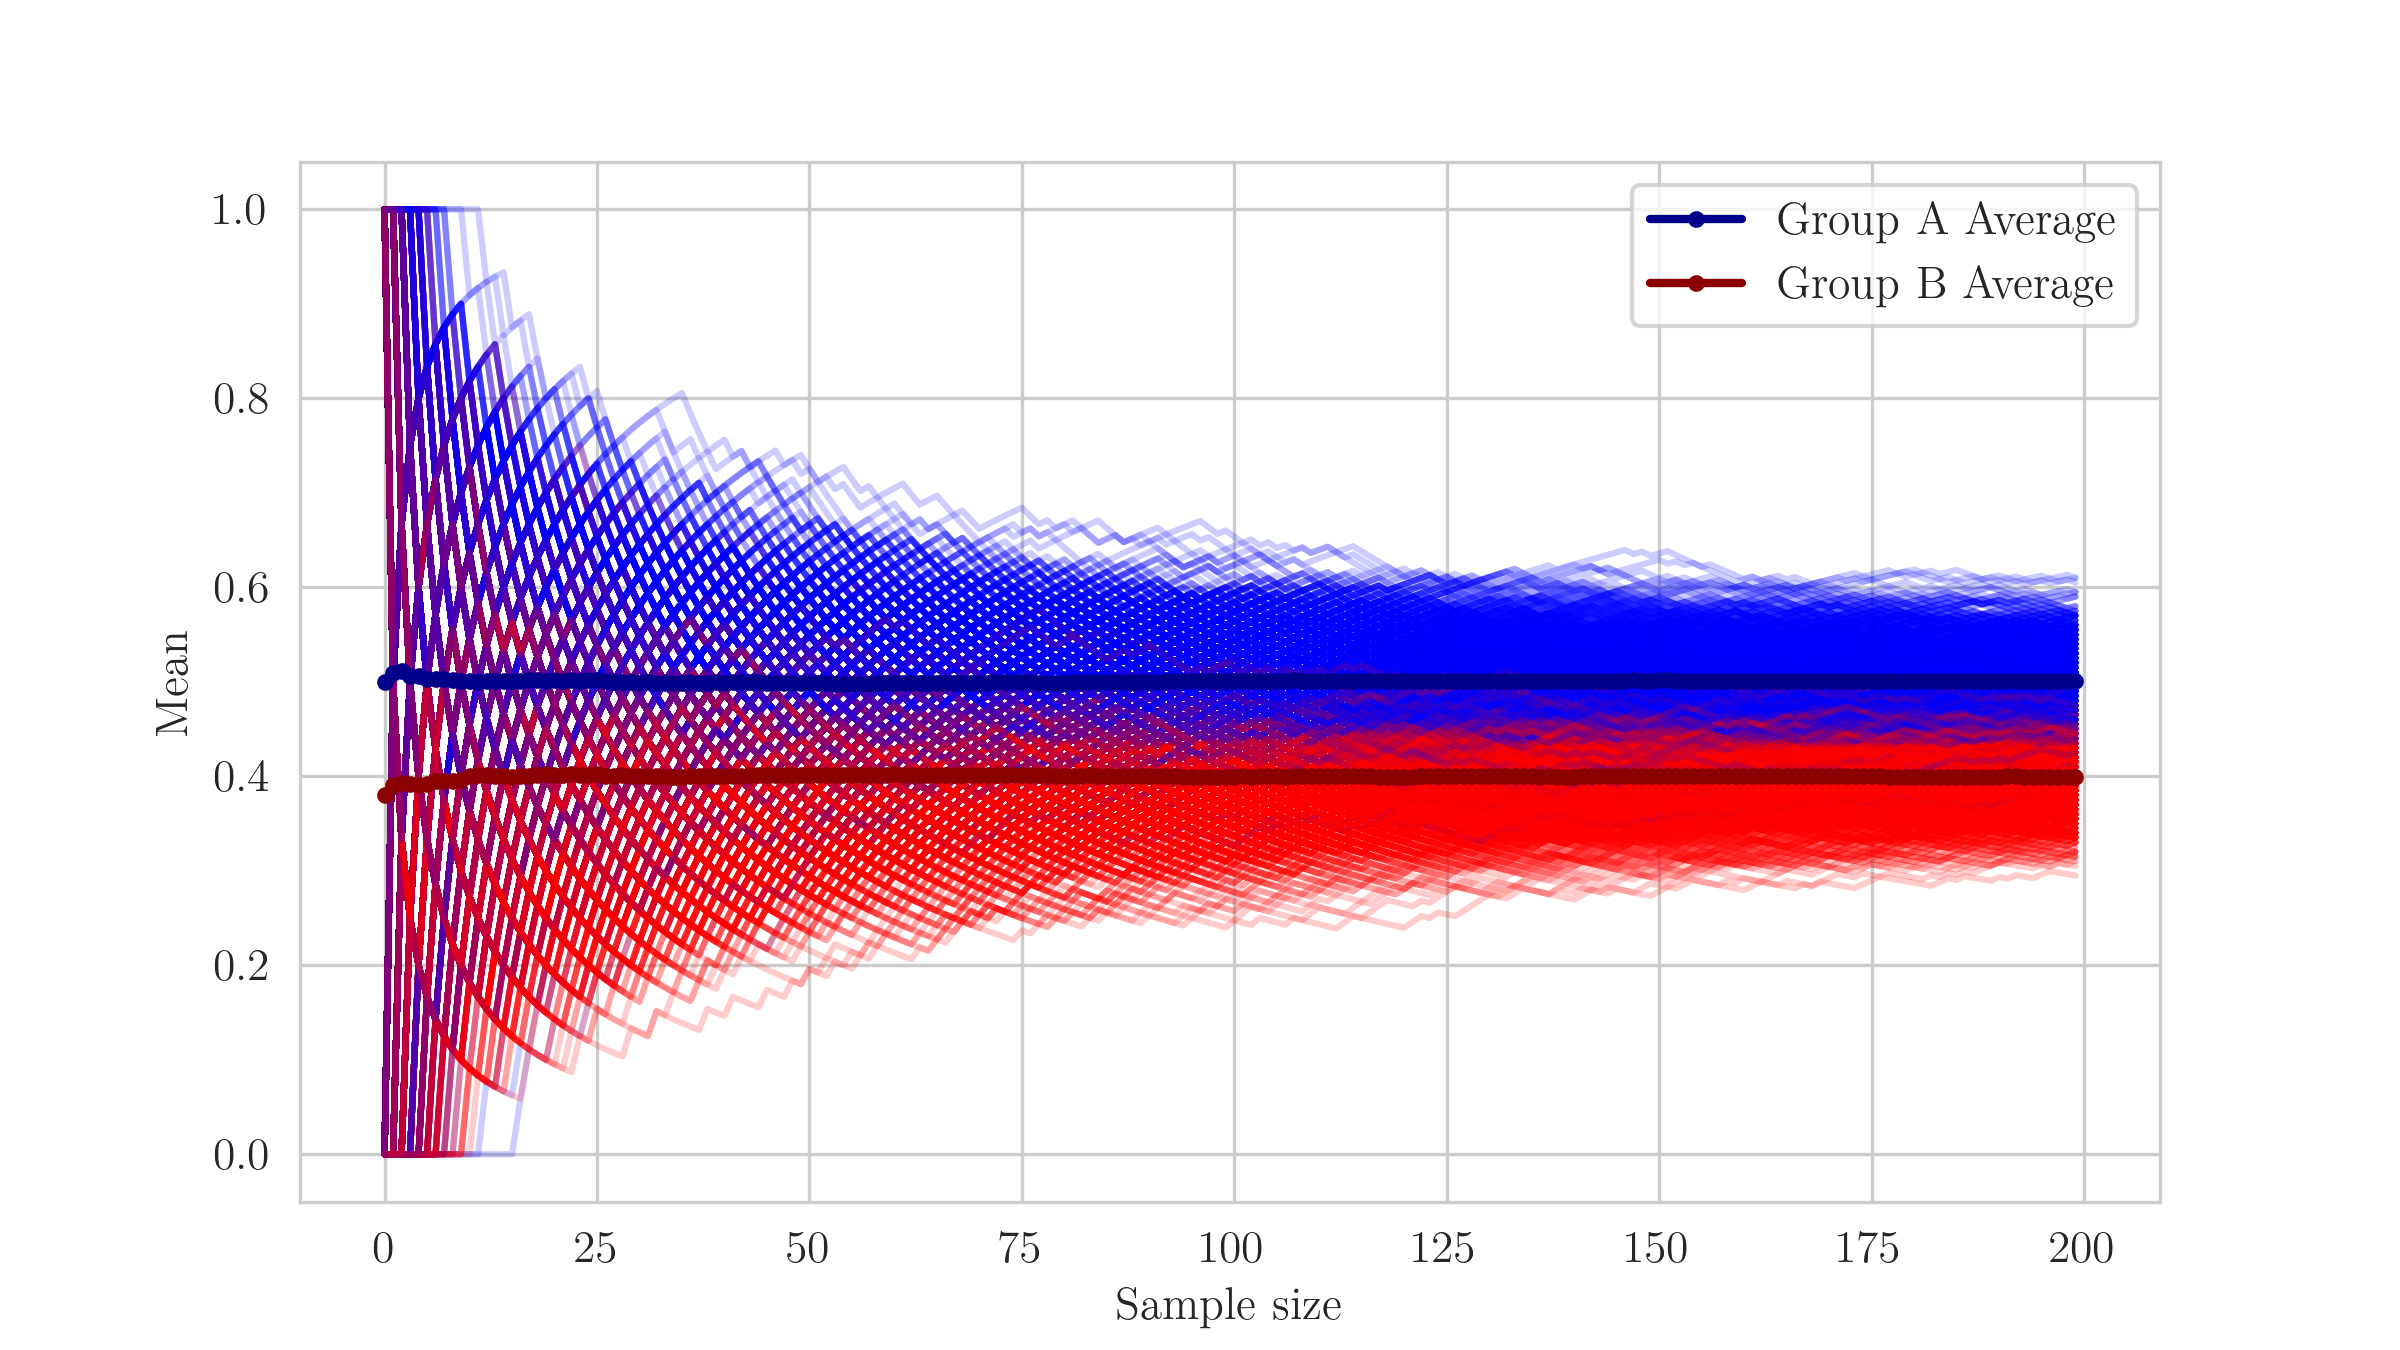
\includegraphics[width=\textwidth]{images/cumulative_means.png}
	\caption{Cumulative means for two groups: Group A with \( p_A = 0.5 \) and Group B with \( p_B = 0.4 \). Each line represents an individual simulation, while the darker lines denote the average trajectory across multiple simulations.}
	\label{fig:cumulative_means}
\end{figure}

\begin{figure}[H]
	\centering
	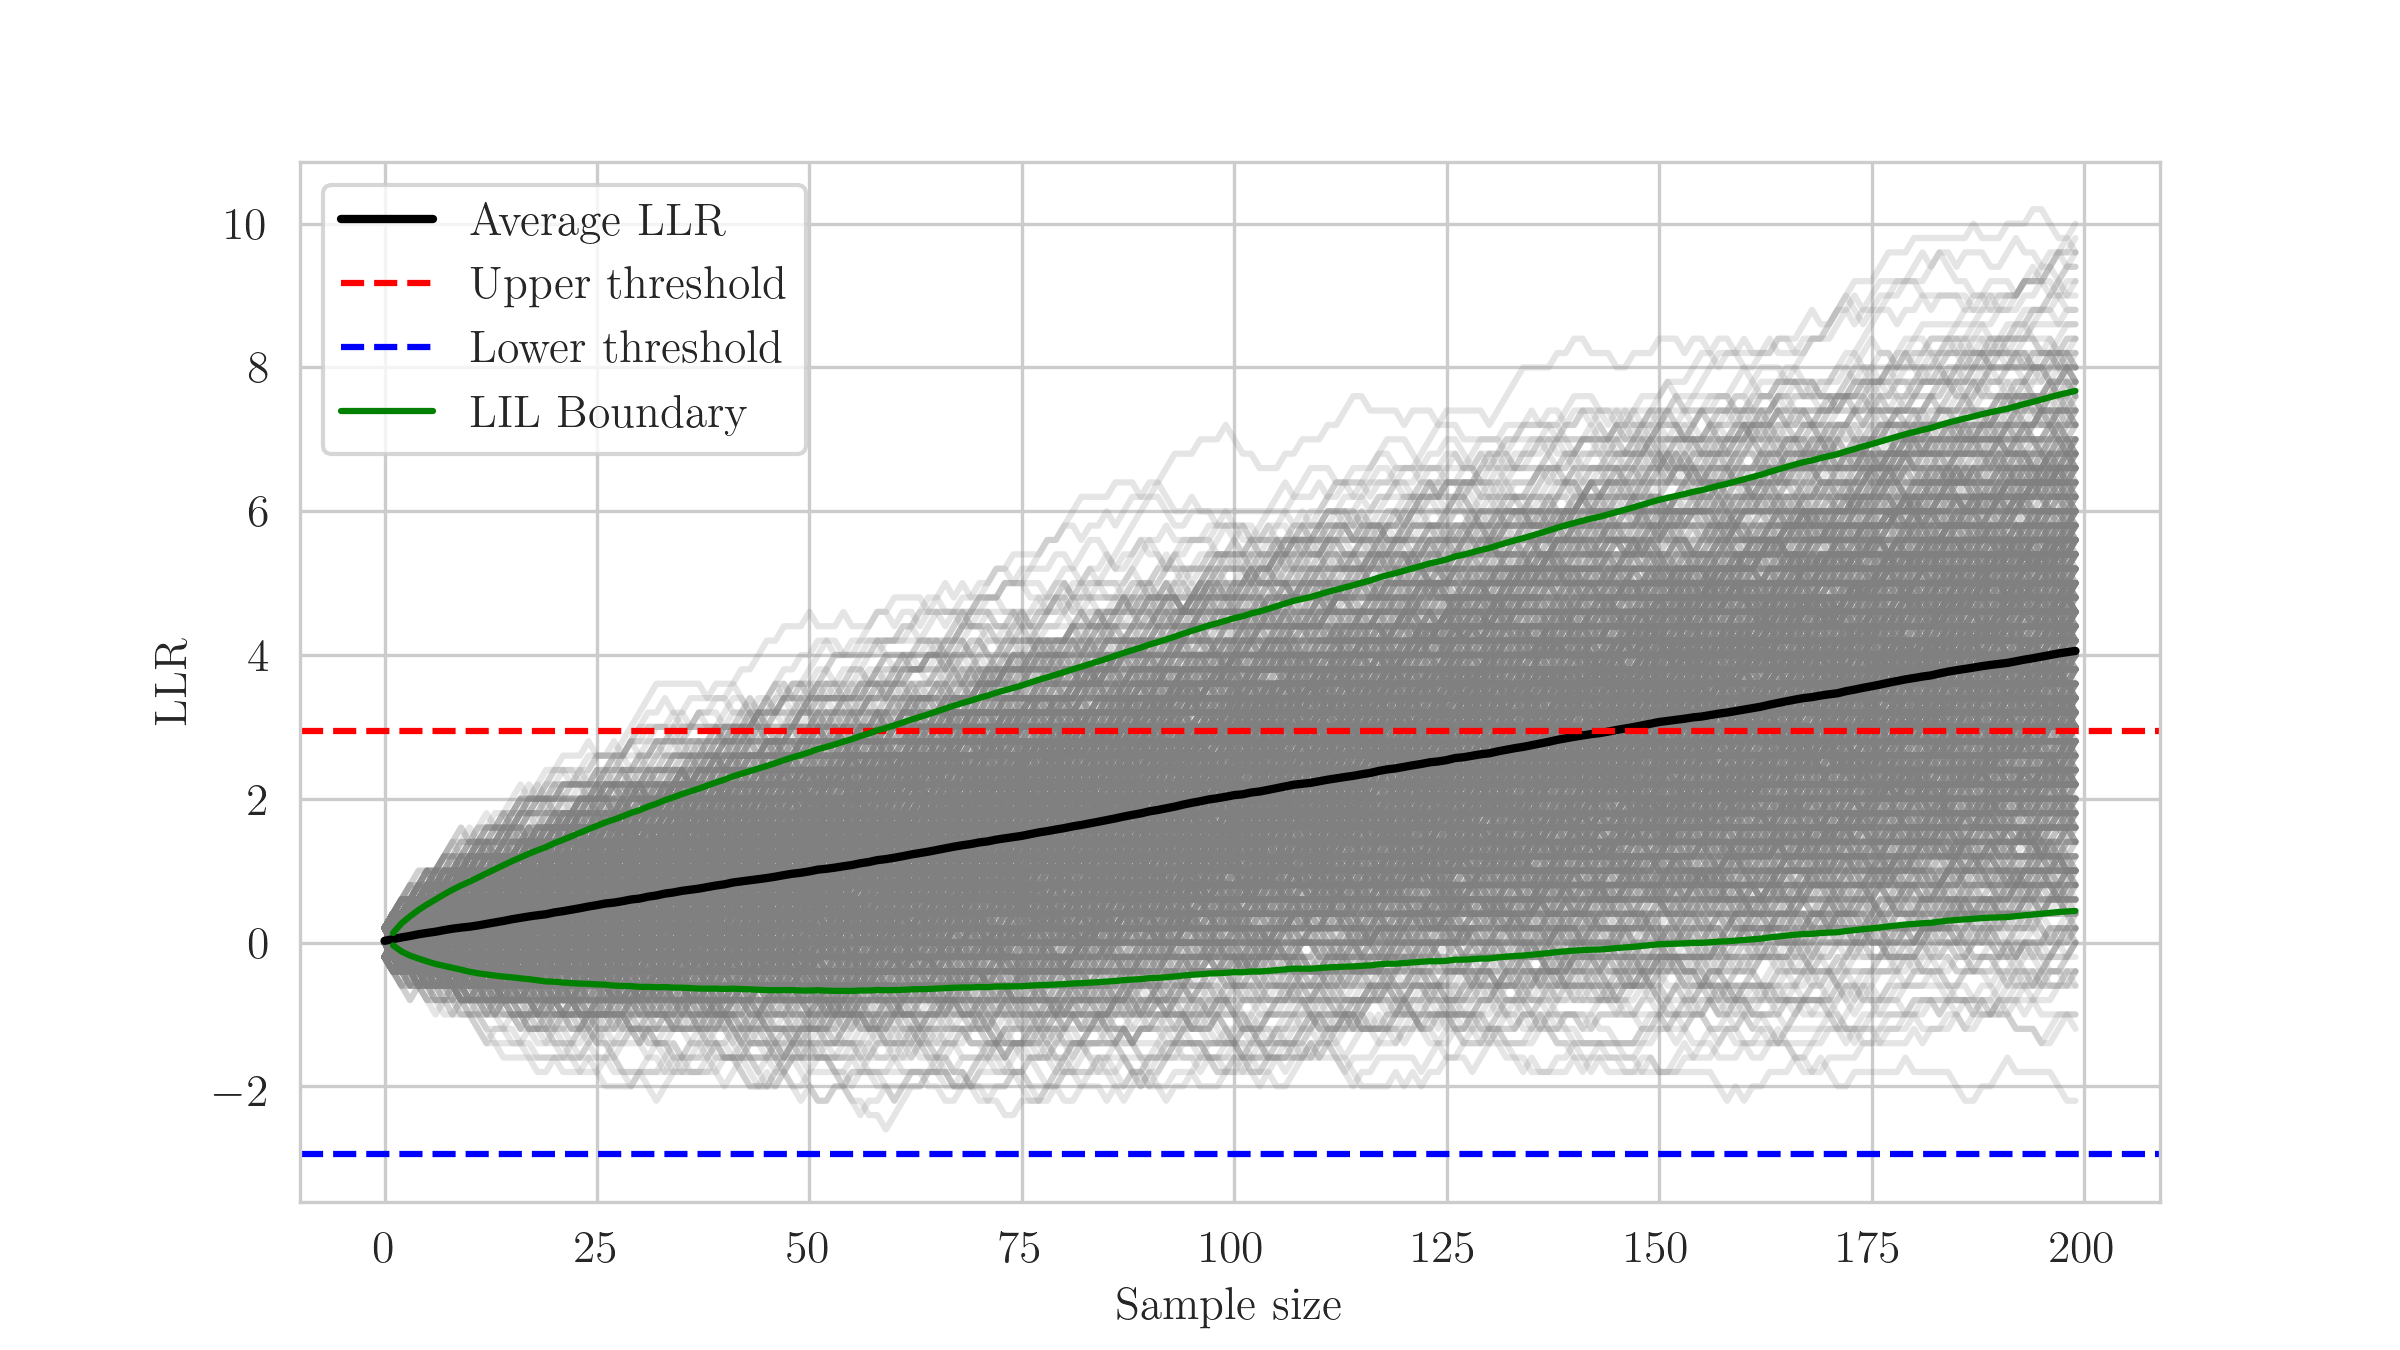
\includegraphics[width=\textwidth]{images/llr_trajectories.png}
	\caption{Log-Likelihood Ratio (LLR) trajectories for the same simulation setup. The~average LLR is depicted in black, with upper and lower decision thresholds indicated by~dashed lines. The green lines represent the Law of the Iterated Logarithm (LIL) boundaries, adjusted for sample size, risk tolerance \(\delta\), and distribution variability.}
	\label{fig:llr_trajectories}
\end{figure}

Figure \ref{fig:llr_trajectories} shows the trajectories of the Log-Likelihood Ratio (LLR) for the same set of~simulations. The grey lines represent the LLR trajectories for individual simulations, while the black line indicates the average LLR across all simulations. The red and blue dashed lines represent the upper and lower decision thresholds, respectively. Additionally,~the green lines depict the Law of the Iterated Logarithm (LIL) boundaries, calculated as:
%TODO moze dowód?
\[
(p_A - p_B) t \delta \pm \sqrt{2t \log(\log(t))} \cdot \sqrt{p_A(1-p_A) + p_B(1-p_B)} \cdot \delta,
\]

where \( t \) represents the sample size, \( p_A \) and \( p_B \) denote the success probabilities of Groups A and B, respectively, and \( \delta \) is the risk tolerance parameter utilized in the simulation. These LIL boundaries provide theoretical constraints on the LLR's behavior, accounting for both sample size and the inherent variability of the distributions.

These simulations vividly illustrate the dynamics of sequential A/B testing, highlighting the potential for early stopping when sufficient evidence is accumulated. The visualizations serve as a foundational demonstration of the efficacy and practical utility of sequential testing methodologies.

\section{Average Stopping Time and Error Rate Analysis}

In this section, we analyze the average stopping time and error rate across various scenarios involving different success probabilities \( p_A \) and \( p_B \) for groups A and B, respectively. These metrics are critical for evaluating the performance of sequential A/B testing, particularly in determining the test's efficiency and accuracy.

\subsection{Simulation Setup}

The simulations were conducted across a range of success probabilities \( p_A \) and \( p_B \),~varying from 0.05 to 0.95 in increments of 0.05. For each pair of probabilities \( (p_A, p_B) \), 1000~simulations were executed. The decision to stop the test was based on the log-likelihood ratio (LLR), with the upper and lower thresholds determined by the significance level \( \alpha = 0.05 \). The risk tolerance parameter \( \delta \) was set to 0.3. During the simulations, both the average stopping time and the error rate were recorded, where the error rate represents the proportion of simulations in which the sequential test incorrectly rejected or accepted the null hypothesis.

\subsection{Average Stopping Time}

Figure \ref{fig:avg_stopping_time} shows the heatmap of the average stopping time as a function of the success probabilities \( p_A \) and \( p_B \). The color intensity corresponds to the average stopping time, with warmer colors indicating longer stopping durations.

%TODO on page dodac tam gdie to ebdzie przydatne
As depicted in Figure \ref{fig:avg_stopping_time}, the average stopping time generally increases as the success probabilities \( p_A \) and \( p_B \) converge. This behavior is anticipated since distinguishing between two groups becomes more challenging when their success probabilities are similar, necessitating more observations to reach a confident conclusion. The red dashed lines represent the risk tolerance boundaries, illustrating the regions where the difference between \( p_A \) and \( p_B \) meets the predefined risk tolerance.
\begin{figure}[H]
	\centering
	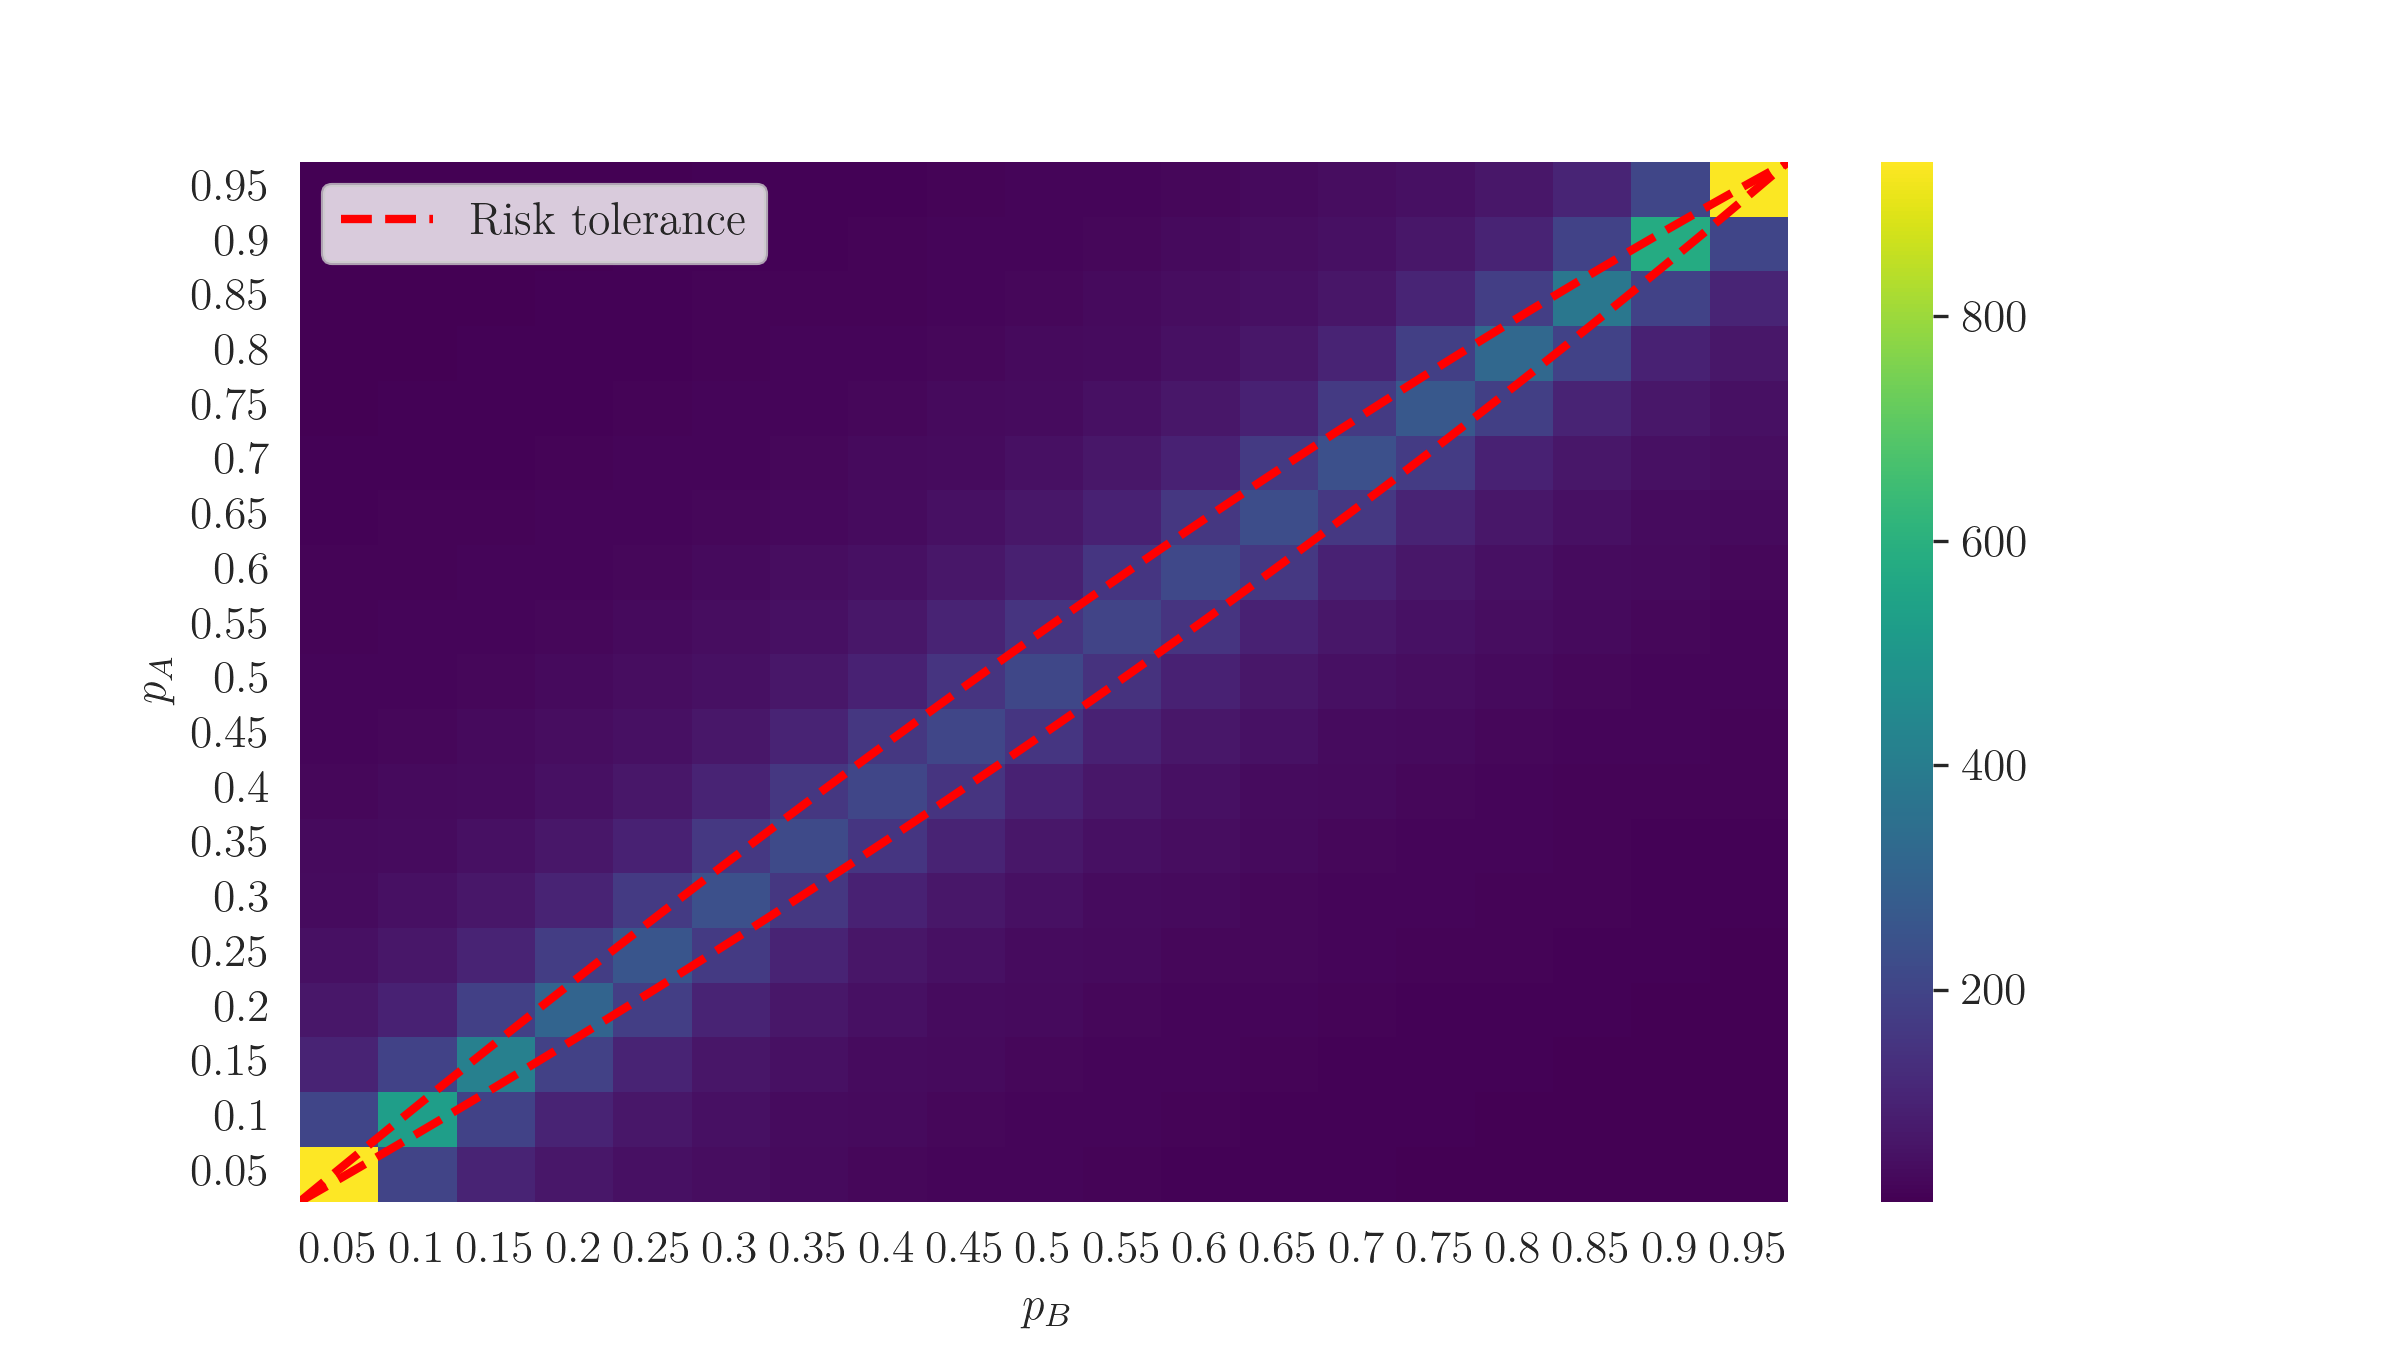
\includegraphics[width=0.9\textwidth]{images/average_stopping_time_matrix.png}
	\caption{Average stopping time as a function of the success probabilities \( p_A \) and \( p_B \). The red dashed lines represent the risk tolerance boundaries, which delineate where the difference between \( p_A \) and \( p_B \) corresponds to the risk level defined by \( \delta \).}
	\label{fig:avg_stopping_time}
\end{figure}

\subsection{Error Rate}
Figure \ref{fig:error_rate} presents the heatmap of the error rate across various combinations of \( p_A \) and \( p_B \). The error rate is computed as the proportion of simulations where the test incorrectly accepted or rejected the null hypothesis.

\begin{figure}[H]
	\centering
	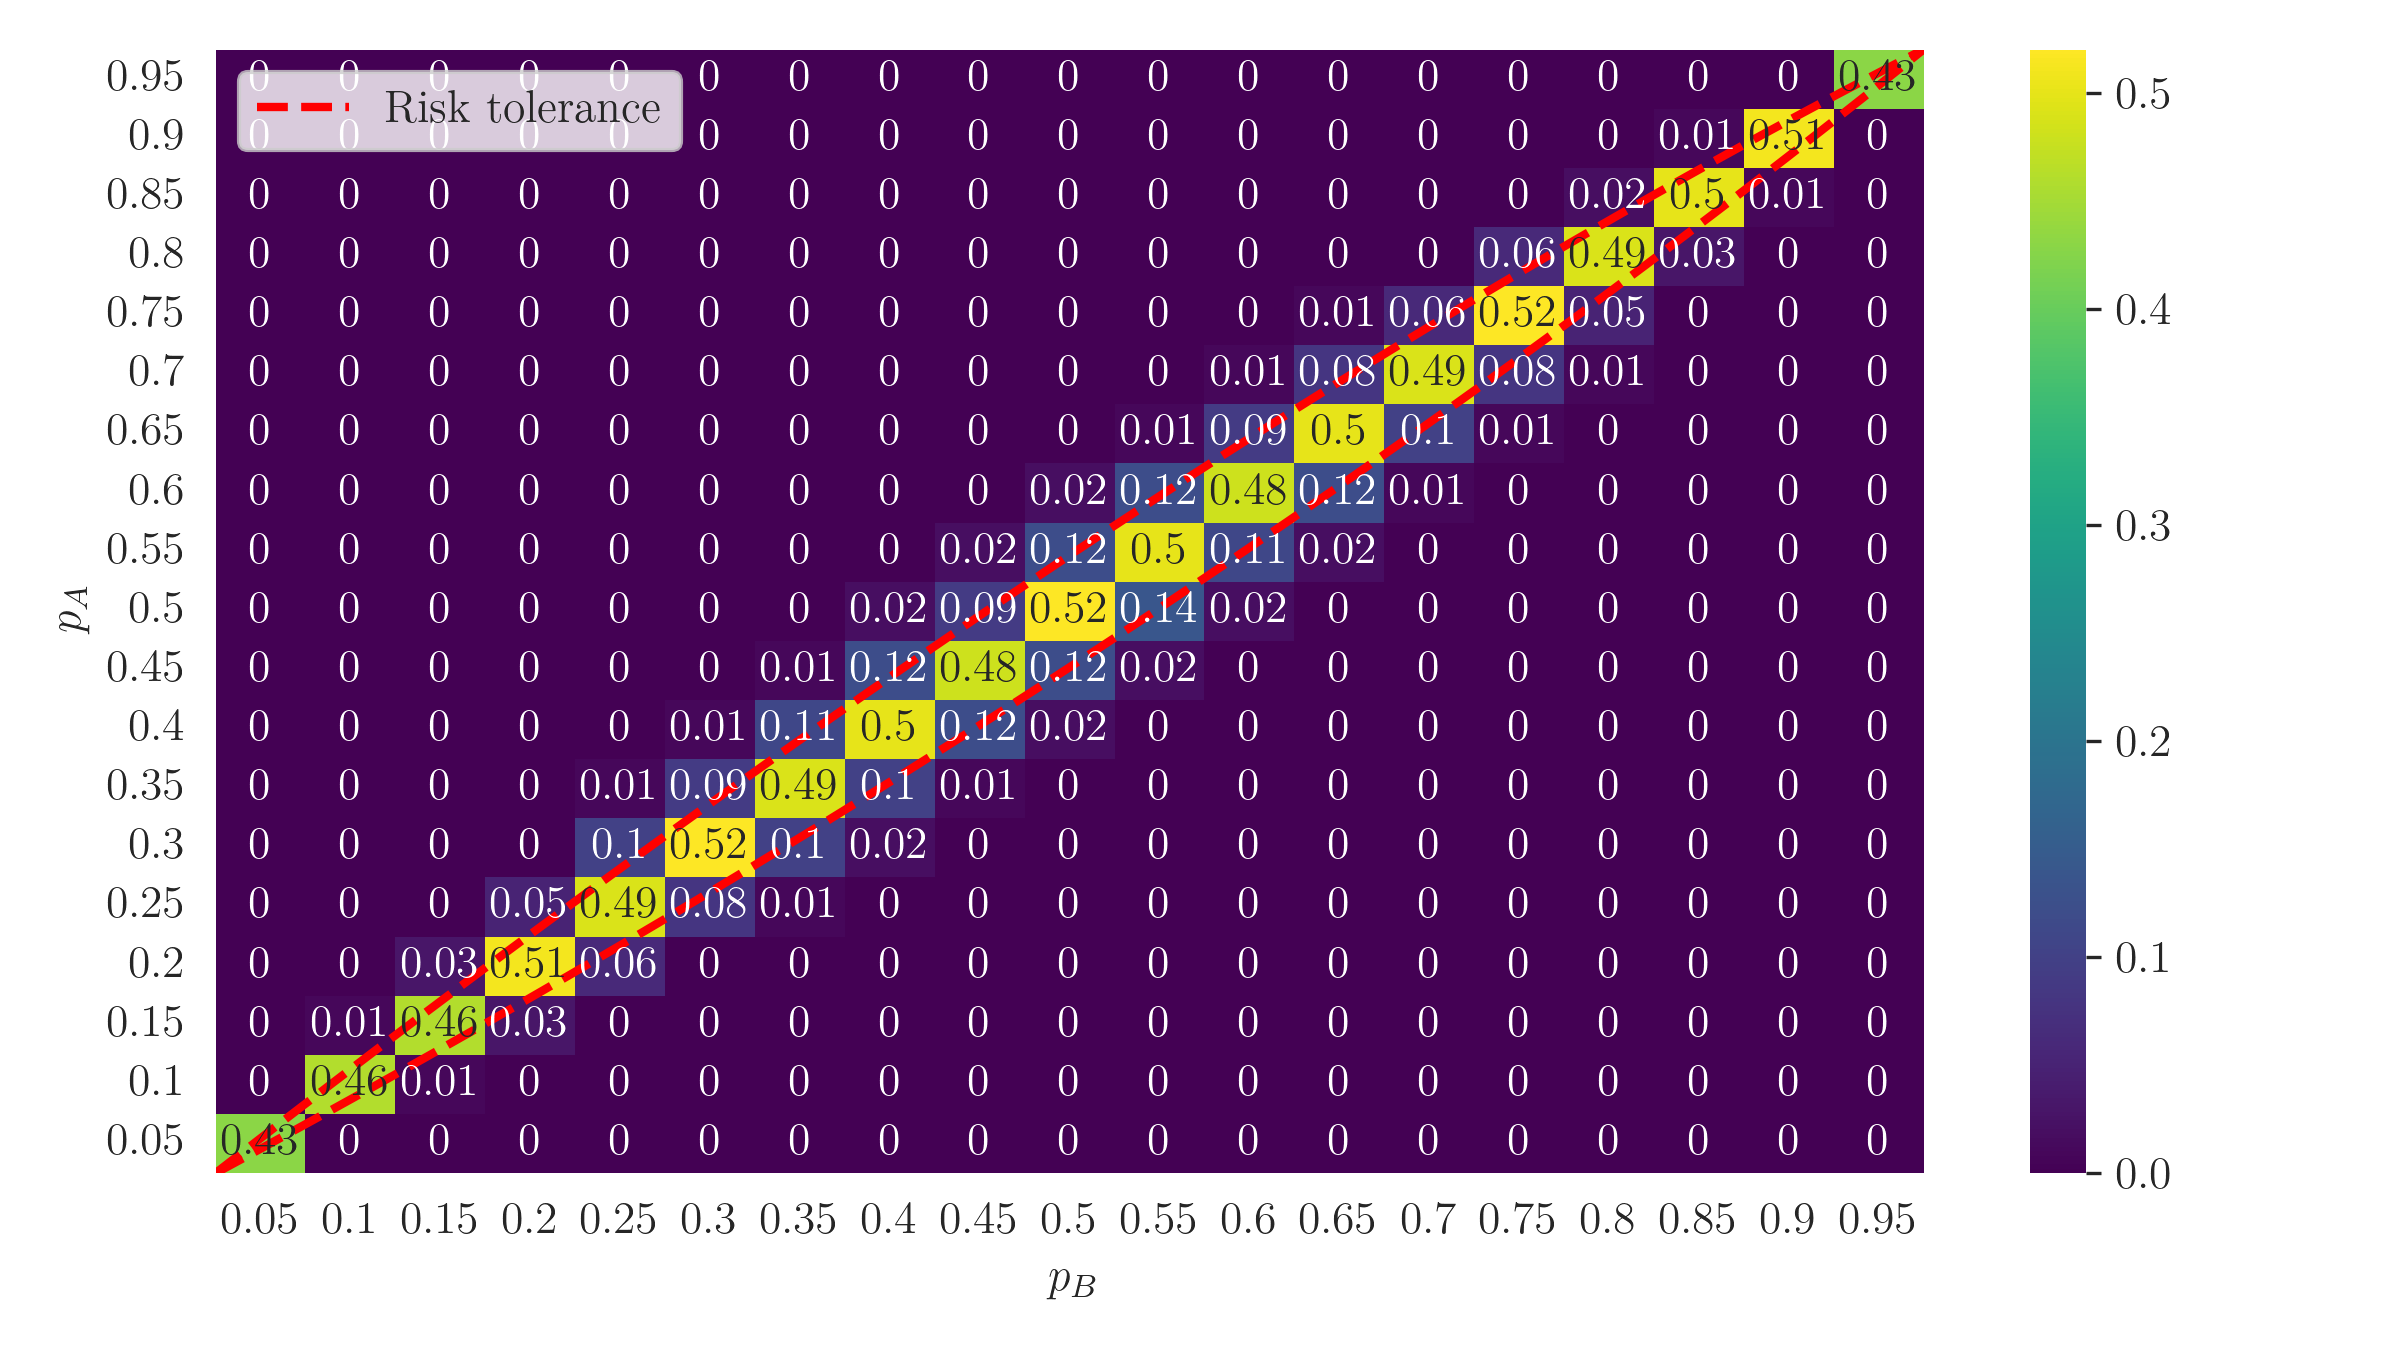
\includegraphics[width=0.9\textwidth]{images/error_rate_matrix.png}
	\caption{Error rate as a function of the success probabilities \( p_A \) and \( p_B \). Warmer colors indicate higher error rates. The red dashed lines represent the risk tolerance boundaries, indicating where the difference between \( p_A \) and \( p_B \) corresponds to the risk level defined by~\( \delta \).}
	\label{fig:error_rate}
\end{figure}

As shown in Figure \ref{fig:error_rate}, the error rate peaks when the success probabilities \( p_A \) and \( p_B \) are nearly equal. This occurs because the closer the success probabilities, the more challenging it becomes for the test to differentiate between the two groups accurately, leading to a higher likelihood of Type I or Type II errors. Conversely, the error rate decreases as the difference between \( p_A \) and \( p_B \) increases, which aligns with the theoretical expectation that tests are more reliable when the effect size is more pronounced.

This analysis underscores the necessity of balancing the trade-offs between the average stopping time and the error rate when designing and interpreting sequential A/B tests. By~understanding these metrics, researchers can make more informed decisions in the context of online experimentation, ensuring efficient use of resources while maintaining rigorous statistical standards.

\section{Detailed Analysis for a 50\% Success Probability}

In this section, we conduct a detailed analysis of the sequential A/B testing performance when the probability of success in Group A is fixed at \( p_A = 0.5 \), and the probability of~success in Group B, \( p_B \), varies. This analysis provides more profound insights into how the sequential test behaves as the success probabilities of the two groups become increasingly similar or dissimilar.

\subsection{Average Stopping Time}

Figure \ref{fig:avg_stopping_time_pa05} illustrates the relationship between \( p_B \) and the average stopping time of~the sequential test. As expected, the average stopping time increases as \( p_B \) approaches \( p_A = 0.5 \). This is because when the success probabilities of the two groups are close, it becomes more challenging for the test to gather enough evidence to decisively favor one group over the other. Consequently, more samples are required, leading to a longer stopping time.

The red dashed lines represent the risk tolerance bounds, indicating the values of~\( p_B \)~where the decision boundaries are most likely to be crossed. Within this range, the test generally requires the maximum number of samples to reach a conclusion.
\begin{figure}[H]
	\centering
	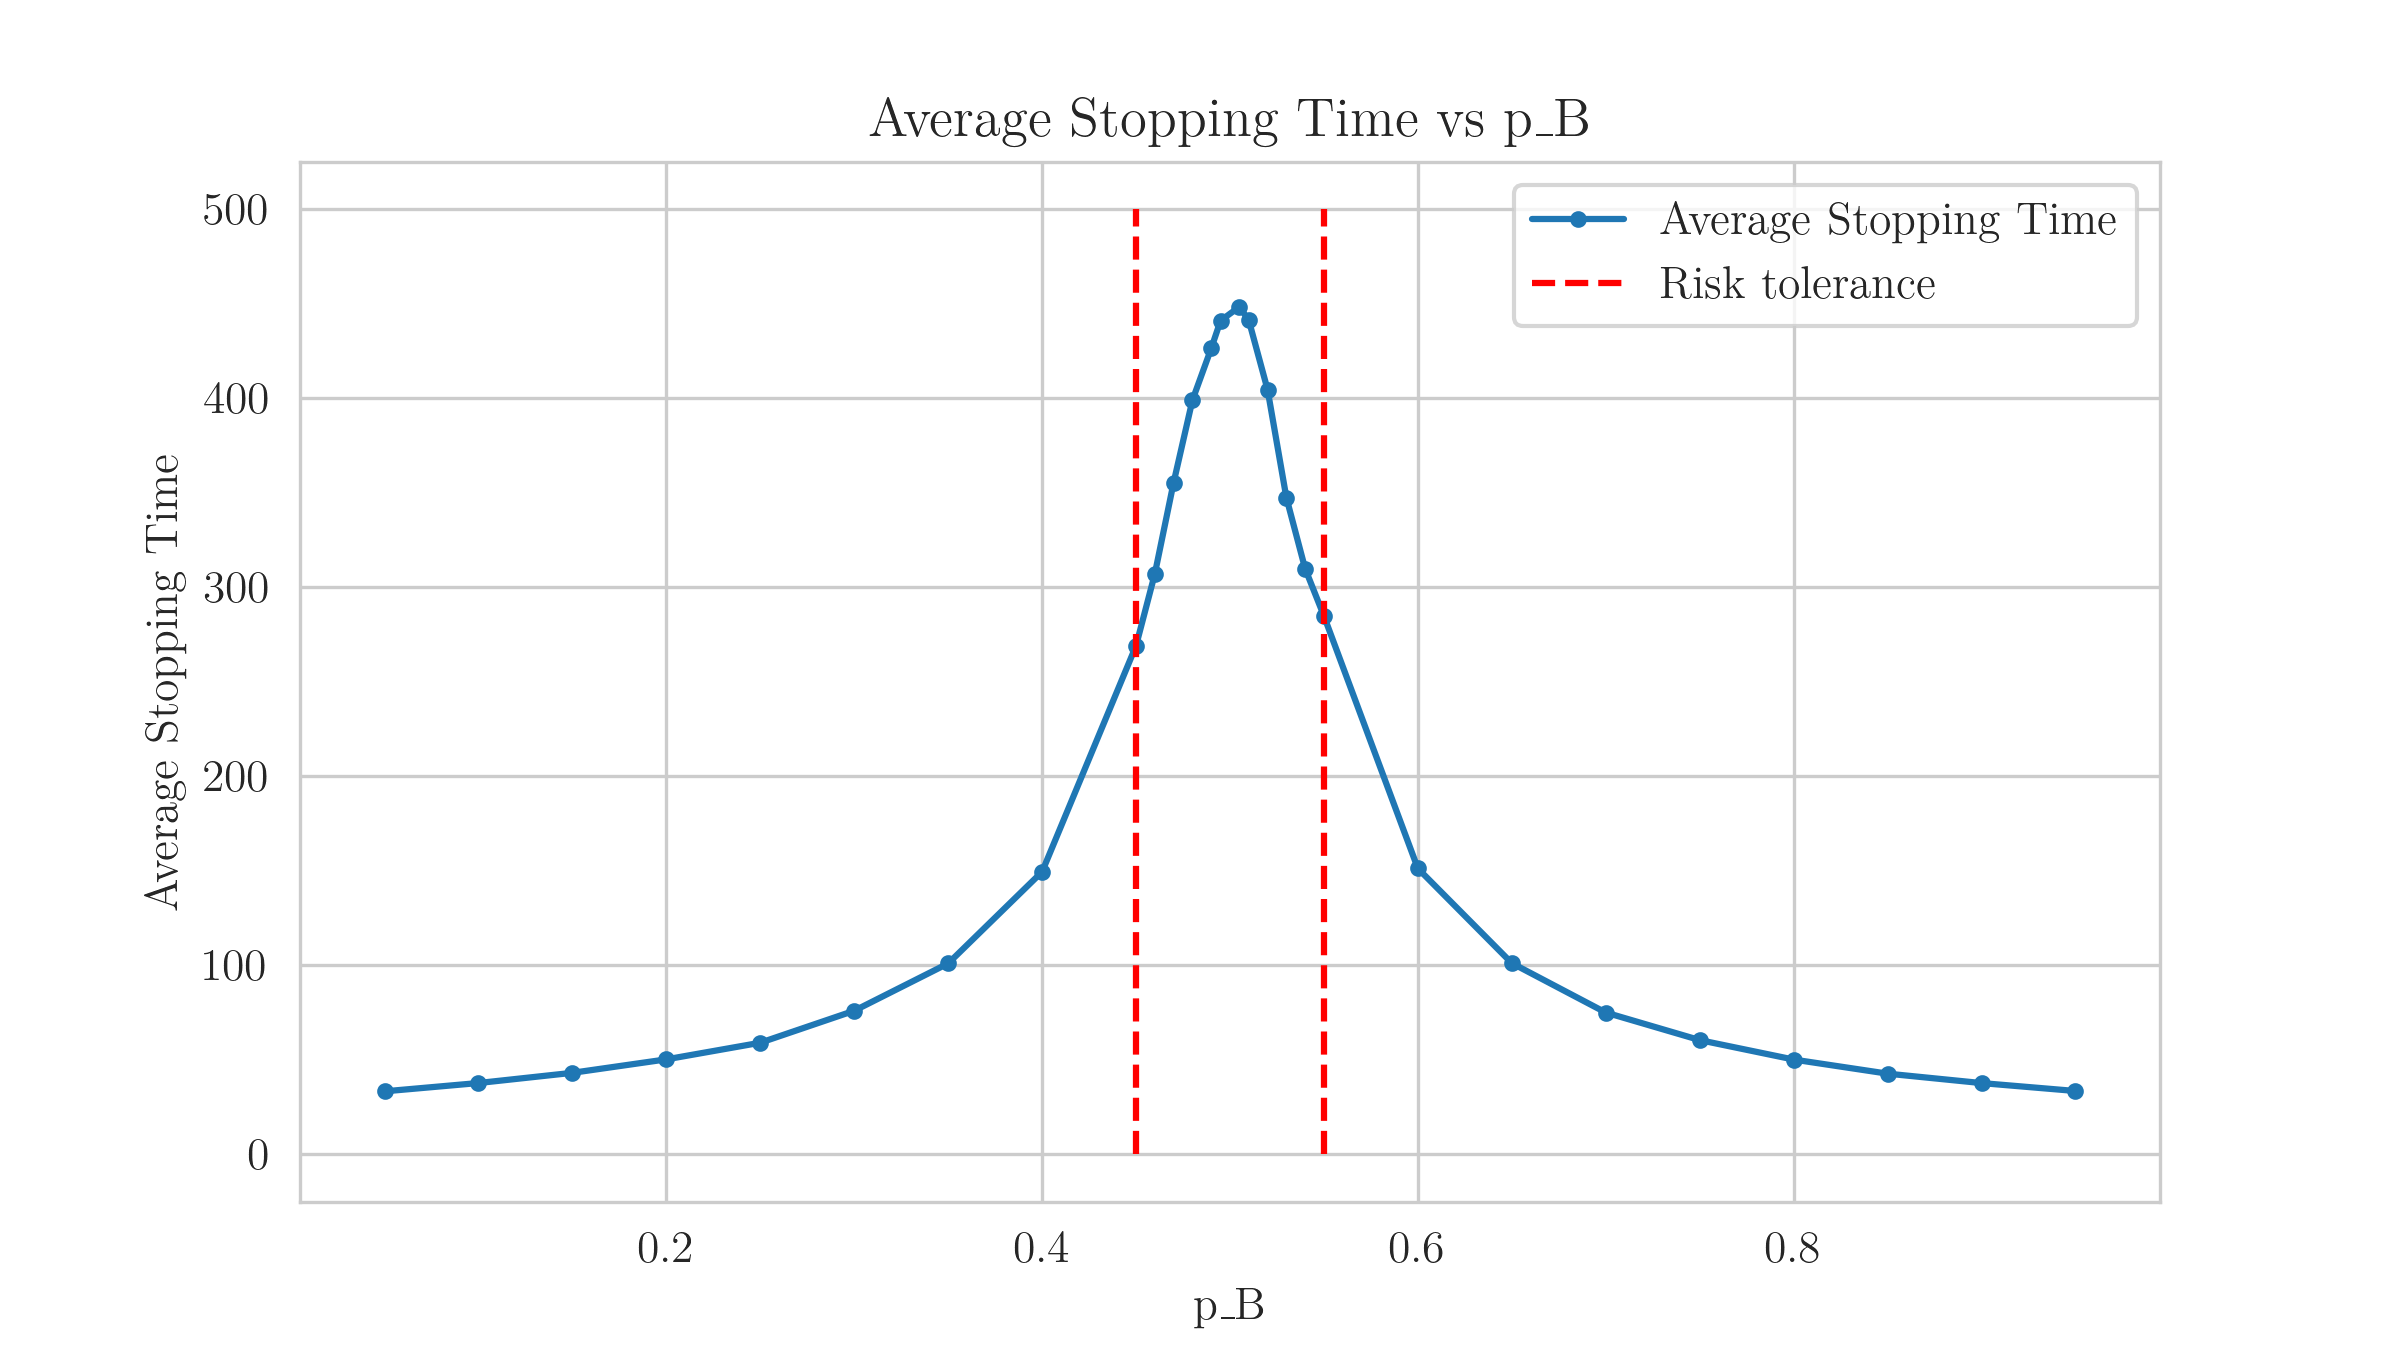
\includegraphics[width=0.8\textwidth]{images/average_stopping_time_pa05.png}
	\caption{Average Stopping Time as a function of \( p_B \) for \( p_A = 0.5 \). The red dashed lines represent the risk tolerance bounds.}
	\label{fig:avg_stopping_time_pa05}
\end{figure}
\subsection{Error Rate Analysis 1}
Figure \ref{fig:error_rate_pa05} shows the error rate as a function of \( p_B \) when the success probability in~Group A is fixed at \( p_A = 0.5 \). The results indicate that the error rate is minimal when \( p_B \)~is substantially different from \( p_A = 0.5 \). This suggests that the sequential test is highly effective at distinguishing between the two groups when there is a significant difference in~their success probabilities.

However, as \( p_B \) approaches \( p_A = 0.5 \), the error rate increases, reaching its peak when \( p_B \) is nearly equal to \( p_A \). This increase in error rate is due to the difficulty of distinguishing between the two groups when their success probabilities are nearly identical. In such cases, the test struggles to accumulate sufficient evidence to confidently reject the null hypothesis, leading to a higher likelihood of errors.

The blue dashed line in Figure \ref{fig:error_rate_pa05} represents the significance level \( \alpha = 0.05 \), which is~the maximum acceptable probability of making a Type I error (false positive). Notably,~the error rate exceeds this threshold near the risk tolerance bounds, highlighting the inherent trade-off between sensitivity and specificity in sequential testing. This trade-off must be~carefully managed, especially in scenarios where the cost of errors is high.

\begin{figure}[H]
	\centering
	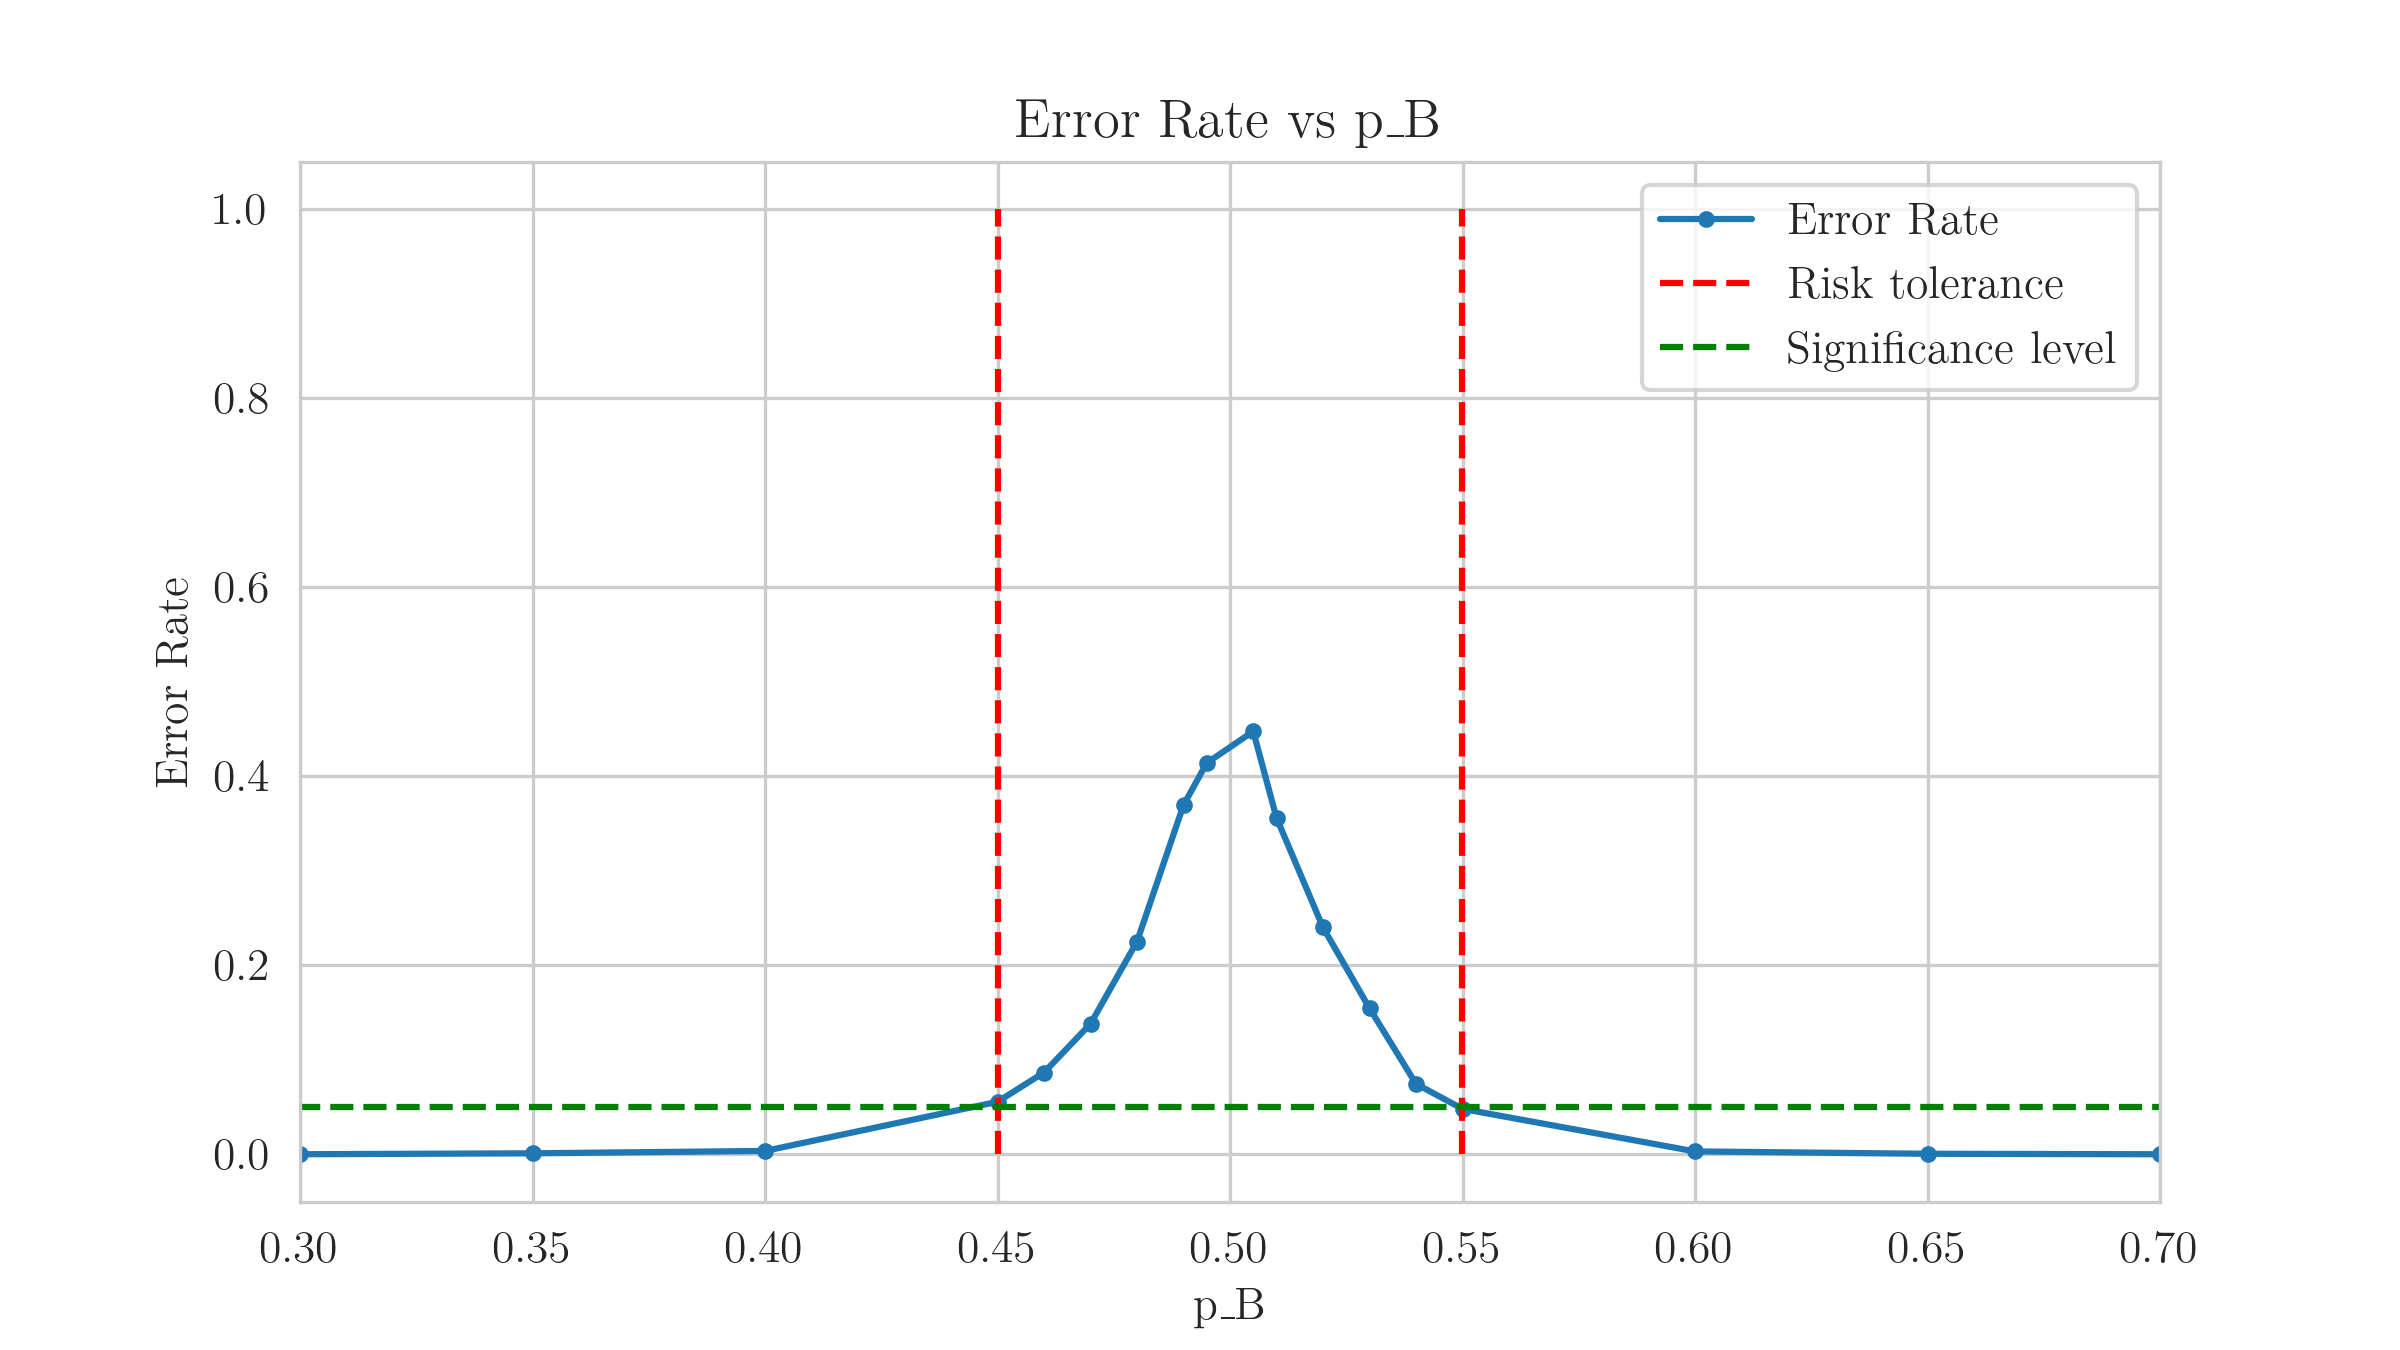
\includegraphics[width=0.9\textwidth]{images/error_rate_pa05.png}
	\caption{Error Rate as a function of \( p_B \) for \( p_A = 0.5 \). The red dashed lines represent the risk tolerance bounds, and the blue dashed line represents the significance level.}
	\label{fig:error_rate_pa05}
\end{figure}

To further clarify the behavior of the test, Table \ref{tab:descriptive_stats} provides descriptive statistics for the stopping times across different values of \( p_B \), along with the corresponding error rates. The data reveals that as \( p_B \) approaches \( p_A \), not only does the error rate increase, but the mean stopping time also lengthens, reflecting the increased difficulty in reaching a~conclusive decision.

\begin{table}[H]
	\centering
	\caption{Descriptive Statistics and Error Rate for Various \( p_B \) Values.}
	\label{tab:descriptive_stats}
	\begin{tabular}{lccccccccc}
		\toprule
		& \multicolumn{9}{c}{\( \mathbf{p_B} \)} \\ \cmidrule(lr){2-10}
		\textbf{Stop time}& 0.1 & 0.2 & 0.3 & 0.4 & 0.45 & 0.47 & 0.48 & 0.49 & 0.495 \\
		\midrule
		\textbf{Mean} & 37.69 & 50.21 & 75.92 & 149.46 & 269.08 & 355.41 & 398.96 & 426.36 & 441.07 \\
		\textbf{Std} & 8.92 & 15.40 & 29.84 & 81.40 & 192.76 & 266.59 & 321.06 & 336.41 & 363.75 \\
		\textbf{Min} & 18 & 19 & 22 & 31 & 34 & 33 & 23 & 37 & 44 \\
		\textbf{25\%} & 31 & 40 & 55 & 91 & 136 & 167 & 179 & 186 & 192 \\
		\textbf{Median} & 37 & 48 & 70 & 130 & 217 & 280 & 298 & 330 & 327 \\
		\textbf{75\%} & 43 & 58 & 91 & 188 & 349 & 459 & 529 & 567 & 580 \\
		\textbf{Max} & 86 & 122 & 232 & 613 & 1672 & 2143 & 2521 & 2445 & 2615 \\
		\hline
		\textbf{Error Rate} & 0 & 0 & 0 & 0 & 0.06 & 0.14 & 0.23 & 0.37 & 0.41 \\
		\bottomrule
	\end{tabular}
	\caption*{\textit{Source: own elaboration}}
\end{table}

The table shows that as \( p_B \) nears \( p_A \), the stopping times become more variable, with the maximum stopping time increasing substantially. This variability highlights the challenges faced by the sequential test in making a decision when the difference between \( p_A \) and \( p_B \) is~minimal. Moreover, the error rate steadily increases as \( p_B \) approaches \( p_A \), emphasizing the importance of understanding the error dynamics when interpreting the results of~sequential A/B tests.

This analysis underscores the critical importance of selecting appropriate test parameters and understanding their implications on both stopping times and error rates. As~the success probabilities of the two groups converge, the sequential test requires more data to~reach a decision, and the likelihood of error increases, which must be carefully considered in the design and interpretation of experiments.

\section{Detailed Analysis for a 50\% Success Probability 2}

\begin{figure}[H]
	\centering
	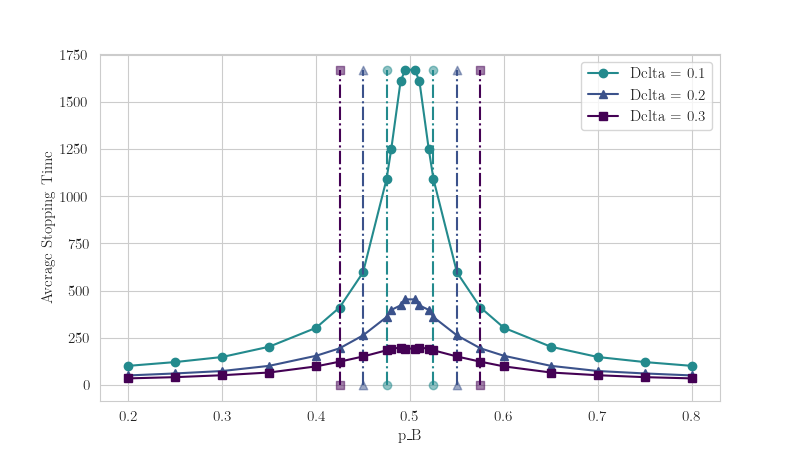
\includegraphics[width=\textwidth]{images/delta_average_stopping_time.png}
	\caption{Average Stopping Time as a function of \( p_B \) for \( p_A = 0.5 \). The dashed lines represent the risk tolerance bounds.}
	\label{fig:avg_stopping_time_pa05}
\end{figure}

\begin{figure}[H]
	\centering
	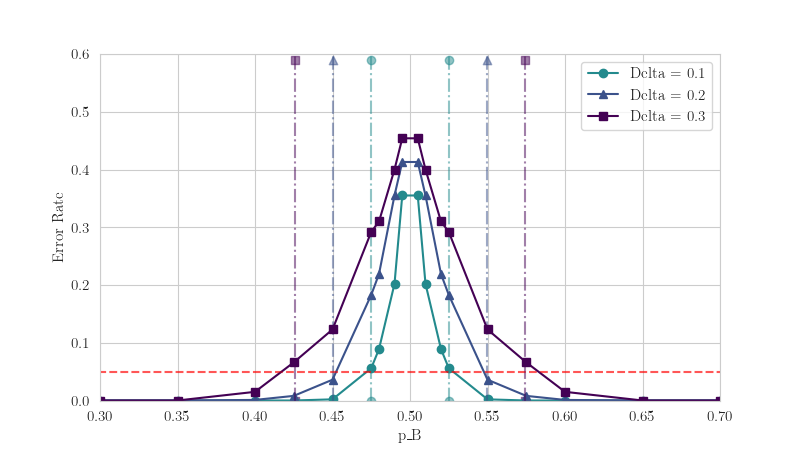
\includegraphics[width=\textwidth]{images/delta_error_rate.png}
	\caption{Error Rate as a function of \( p_B \) for \( p_A = 0.5 \). The red dashed lines represent the risk tolerance bounds, and the blue dashed line represents the significance level.}
	\label{fig:error_rate_pa05}
\end{figure}


\begin{table}
	\centering
	\caption{Descriptive Statistics and Error Rate}
	\label{tab:descriptive_stats}
	\begin{tabular}{llcccccccc}
		\toprule
		& \multicolumn{8}{c}{$p_B$} \\ \cmidrule(lr){2-9}
		& 0.2 & 0.3 & 0.4 & 0.425 & 0.45 & 0.475 & 0.49 & 0.495 \\
		\midrule
		\textbf{mean} & 91.40 & 142 & 329.40 & 330.30 & 452.60 & 1225.80 & 1565 & 2056.10 \\
		\textbf{std} & 14.46 & 37.82 & 116.20 & 118.38 & 131.35 & 697.21 & 1360.89 & 1194.56 \\
		\textbf{min} & 69 & 95 & 132 & 191 & 312 & 400 & 256 & 724 \\
		\textbf{25\%} & 86.25 & 108 & 259.75 & 277.50 & 370.25 & 867 & 925.75 & 1132.75 \\
		\textbf{50\%} & 87.50 & 138 & 315.50 & 307 & 423 & 1101 & 1184 & 1558 \\
		\textbf{75\%} & 97 & 172.75 & 385.25 & 369.25 & 488.50 & 1231.75 & 1811.75 & 3209.50 \\
		\textbf{max} & 120 & 196 & 521 & 582 & 773 & 2489 & 5000 & 3710 \\
		\textbf{Error Rate} & 0 & 0 & 0 & 0 & 0.00 & 0.06 & 0.20 & 0.35 \\
		\bottomrule
	\end{tabular}
\end{table}

\begin{table}
	\centering
	\caption{Descriptive Statistics and Error Rate}
	\label{tab:descriptive_stats}
	\begin{tabular}{llcccccccc}
		\toprule
		& \multicolumn{8}{c}{$p_B$} \\ \cmidrule(lr){2-9}
		& 0.2 & 0.3 & 0.4 & 0.425 & 0.45 & 0.475 & 0.49 & 0.495 \\
		\midrule
		\textbf{mean} & 41.60 & 82.80 & 160.40 & 226.90 & 256 & 356.40 & 323.60 & 347.40 \\
		\textbf{std} & 11.55 & 24.67 & 122.09 & 141.22 & 94.50 & 143.24 & 280.86 & 232.70 \\
		\textbf{min} & 25 & 55 & 69 & 108 & 84 & 105 & 97 & 53 \\
		\textbf{25\%} & 31.75 & 68 & 92 & 149.50 & 187.75 & 308 & 155.50 & 122.50 \\
		\textbf{50\%} & 41 & 79.50 & 118.50 & 184 & 258 & 345 & 239 & 371.50 \\
		\textbf{75\%} & 52.50 & 87 & 139.75 & 206.25 & 336 & 413 & 329.25 & 513.25 \\
		\textbf{max} & 57 & 145 & 432 & 537 & 363 & 590 & 1032 & 705 \\
		\textbf{Error Rate} & 0 & 0 & 0.00 & 0.01 & 0.04 & 0.18 & 0.35 & 0.41 \\
		\bottomrule
	\end{tabular}
\end{table}

\begin{table}
	\centering
	\caption{Descriptive Statistics and Error Rate}
	\label{tab:descriptive_stats}
	\begin{tabular}{llcccccccc}
		\toprule
		& \multicolumn{8}{c}{$p_B$} \\ \cmidrule(lr){2-9}
		& 0.2 & 0.3 & 0.4 & 0.425 & 0.45 & 0.475 & 0.49 & 0.495 \\
		\midrule
		\textbf{mean} & 34.30 & 38.90 & 129.50 & 112.40 & 204 & 242 & 209.50 & 129.90 \\
		\textbf{std} & 10.49 & 18.12 & 57.75 & 46.75 & 197.23 & 171.60 & 79.28 & 99.85 \\
		\textbf{min} & 17 & 18 & 39 & 40 & 49 & 64 & 52 & 29 \\
		\textbf{25\%} & 28.25 & 29.25 & 81.50 & 71.75 & 87.50 & 142.50 & 177 & 68.50 \\
		\textbf{50\%} & 33 & 32 & 154 & 130 & 136 & 179.50 & 193 & 96 \\
		\textbf{75\%} & 40.25 & 51.75 & 174.75 & 149 & 198.75 & 345.25 & 257.75 & 188 \\
		\textbf{max} & 53 & 68 & 190 & 168 & 672 & 583 & 338 & 349 \\
		\textbf{Error Rate} & 0 & 0 & 0.01 & 0.07 & 0.12 & 0.29 & 0.40 & 0.45 \\
		\bottomrule
	\end{tabular}
\end{table}





\section{Detailed Analysis for a 50\% Success Probability 2}

In this section, we provide a comprehensive analysis of the average stopping time and error rate when the success probability \( p_A \) is fixed at 50\%, while \( p_B \) varies. The analysis incorporates simulations for three different values of the delta parameter: \( \delta = 0.1 \), \( \delta = 0.2 \), and \( \delta = 0.3 \). These delta values represent varying levels of risk tolerance, impacting the speed and accuracy of the sequential A/B testing process.

\subsection{Average Stopping Time Analysis}

\begin{figure}[H]
	\centering
	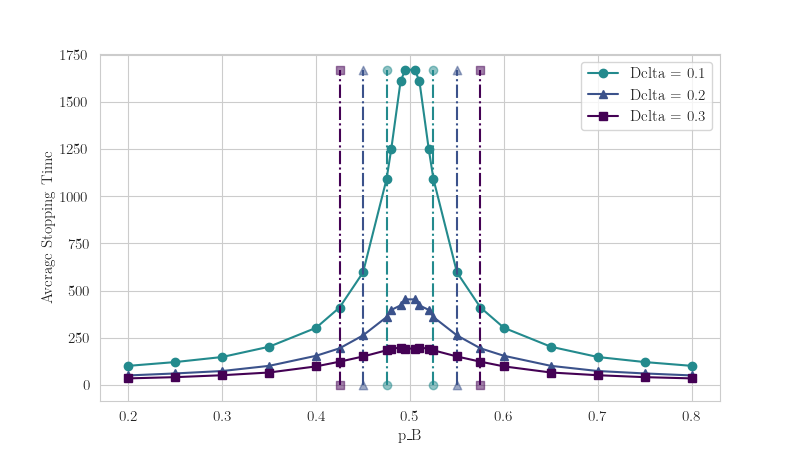
\includegraphics[width=\textwidth]{images/delta_average_stopping_time.png}
	\caption{Average Stopping Time as a function of \( p_B \) for \( p_A = 0.5 \). The dashed lines represent the risk tolerance bounds.}
	\label{fig:avg_stopping_time_pa05}
\end{figure}

Figure \ref{fig:avg_stopping_time_pa05} illustrates the average stopping time as a function of \( p_B \) for three different delta values. The plots clearly demonstrate that smaller delta values, such as \( \delta = 0.1 \), result in significantly longer stopping times, especially as \( p_B \) approaches 0.5. This is because a smaller delta value requires stronger evidence to make a decision, leading to more cautious and prolonged testing.

As the delta value increases to 0.2 and 0.3, the average stopping time decreases across all values of \( p_B \). This reduction is most noticeable when \( p_B \) is close to \( p_A \), reflecting the faster decision-making process due to the looser decision boundaries. However, this comes at the cost of potentially higher error rates, as discussed in the following section.

\subsection{Error Rate Analysis}

\begin{figure}[H]
	\centering
	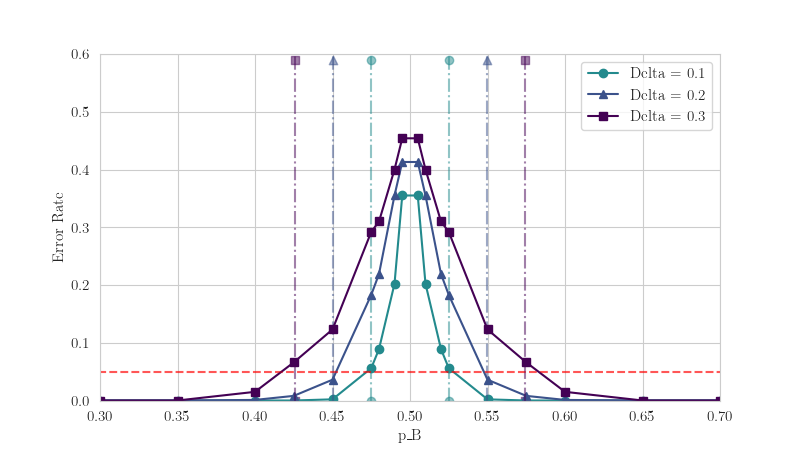
\includegraphics[width=\textwidth]{images/delta_error_rate.png}
	\caption{Error Rate as a function of \( p_B \) for \( p_A = 0.5 \). The red dashed line represents the significance level, and the colored dashed lines represent the risk tolerance bounds for different deltas.}
	\label{fig:error_rate_pa05}
\end{figure}

Figure \ref{fig:error_rate_pa05} shows the error rate as a function of \( p_B \) for the three delta values. As expected, larger delta values correspond to higher error rates, particularly when \( p_B \) is close to \( p_A = 0.5 \). This is because larger deltas allow for faster decisions with less evidence, increasing the likelihood of making an incorrect decision.

The red dashed line represents the significance level, which provides a baseline for acceptable error rates. For smaller delta values like \( \delta = 0.1 \), the error rate remains below this threshold for most values of \( p_B \), indicating a more conservative and reliable testing approach. However, for \( \delta = 0.3 \), the error rate exceeds this threshold as \( p_B \) approaches 0.5, highlighting the trade-off between speed and accuracy.

\subsection{Descriptive Statistics}

The tables below provide detailed descriptive statistics for the stopping times and error rates for different \( p_B \) values and delta settings. These statistics offer a granular view of the simulation results, showcasing the distribution of stopping times and the corresponding error rates.

- **Table 1** shows statistics for \( \delta = 0.1 \).
- **Table 2** shows statistics for \( \delta = 0.2 \).
- **Table 3** shows statistics for \( \delta = 0.3 \).

These tables indicate that as \( p_B \) approaches \( p_A \), the mean stopping time and the variability (as measured by the standard deviation) increase. The error rate also tends to rise, especially for higher delta values, reaffirming the trade-off between speed and accuracy in sequential testing.

\subsection{Summary}

This analysis demonstrates the complex interplay between delta values, stopping times, and error rates in sequential A/B testing. Selecting an appropriate delta is crucial, as it balances the need for quick decision-making against the risk of errors. The results emphasize that while larger delta values can significantly reduce average stopping times, they do so at the cost of higher error rates. Therefore, the choice of delta should be carefully aligned with the specific goals and constraints of the testing scenario.



{\backmatter \chapter{Summary}}

This thesis investigates sequential A/B testing, an advanced methodology that improves upon traditional fixed-sample A/B tests by allowing continuous data evaluation and adaptive decision-making. The core theoretical concepts, including the Sequential Probability Ratio Test (SPRT) and its extension, are analyzed to demonstrate their advantages in~controlling error rates and optimizing experiment duration.

Through simulations, the thesis illustrates how sequential methods enable earlier and more efficient decision-making, especially when differences between variants are subtle. The~results show that these methods significantly reduce average stopping times and error rates compared to classical approaches. Additionally, the practical challenges of implementing sequential testing in real-world environments, such as the need for sophisticated technical infrastructure and rigorous error control, are addressed.

In conclusion, sequential A/B testing offers a powerful alternative to classical methods, particularly in contexts requiring quick and reliable decision-making. The findings suggest that these methods hold great potential for broader application in both research and industry, providing a more efficient and accurate approach to experimental design.


%\appendix 
\backmatter \chapter{Appendix} \label{Appendix}
\setcounter{chapter}{1}
\setcounter{section}{0}
\renewcommand{\thesection}{\Alph{chapter}.\arabic{section}}
\section{Proof of Lemma \ref{lem:sample_size}}\label{proof:sample_size}
\begin{proof}	
	To achieve the desired power \( 1-\beta \) when there is a true difference \( \Delta = p_A - p_B \), the test statistic \( Z \) \eqref{eqn:Z_statistic} under the alternative hypothesis \( H_1 \) should exceed the critical value \( Z_{1-\alpha/2} \). This requirement can be written as:
	\[
	\frac{\Delta}{\sqrt{\frac{p_A(1 - p_A) + p_B(1 - p_B)}{n}}} \geq Z_{1-\alpha/2} + Z_{1-\beta}.
	\]
	Multiplying both sides by the denominator, we obtain:
	\[
	\Delta \geq \left(Z_{1-\alpha/2} + Z_{1-\beta}\right) \sqrt{\frac{p_A(1 - p_A) + p_B(1 - p_B)}{n}}.
	\]
	Rearranging to solve for \( n \), we get:
	\[
	n \geq \frac{(Z_{1-\alpha/2} + Z_{1-\beta})^2 \left(p_A(1 - p_A) + p_B(1 - p_B)\right)}{\Delta^2}.
	\]
	Assuming \( \Delta = p_A - p_B \), the formula simplifies to:
	\[
	n = \frac{(Z_{1-\alpha/2} + Z_{1-\beta})^2 \left(p_A(1 - p_A) + p_B(1 - p_B)\right)}{(p_A - p_B)^2}.
	\]
	Alternatively, this can be rewritten with \( (Z_{\alpha/2} + Z_{\beta})^2 \) as:
	\[
	n = \frac{(Z_{\alpha/2} + Z_{\beta})^2 \left(p_A(1 - p_A) + p_B(1 - p_B)\right)}{(p_A - p_B)^2}.
	\]
	This formula provides the required sample size for each group in an A/B test, ensuring the specified significance level and power.
\end{proof}
\newpage
\section{Proof of normal probability ratio test statistic}\label{proof:normal_prts}


\begin{proof}[Proof of Equation \eqref{eqn:normal_prts}]
	
	Given that the observations \(x_i\) and \(y_i\) are normally distributed with the same variance \(\sigma^2\) but different means \(\mu_1 = \theta_1\) and \(\mu_2 = \theta_2\), we start by considering the probability density functions (PDFs) for \(x_i\) and \(y_i\):
	\[
	f_{\theta_1}(x_i) = \frac{1}{\sqrt{2\pi\sigma^2}} \exp\left(-\frac{(x_i - \theta_1)^2}{2\sigma^2}\right),
	\]
	\[
	f_{\theta_2}(y_i) = \frac{1}{\sqrt{2\pi\sigma^2}} \exp\left(-\frac{(y_i - \theta_2)^2}{2\sigma^2}\right).
	\]
	
	The probability ratio test statistic after \(t\) pairs of data is given by:
	\[
	\frac{p_1^t}{p_0^t} = \prod_{i=1}^{t} \frac{f_{\theta_2}(x_i) f_{\theta_1}(y_i)}{f_{\theta_1}(x_i) f_{\theta_2}(y_i)}.
	\]
	
	Substituting the PDFs into the ratio:
	\[
	\frac{p_1^t}{p_0^t} = \prod_{i=1}^{t} \frac{\frac{1}{\sqrt{2\pi\sigma^2}} \exp\left(-\frac{(x_i - \theta_2)^2}{2\sigma^2}\right) \cdot \frac{1}{\sqrt{2\pi\sigma^2}} \exp\left(-\frac{(y_i - \theta_1)^2}{2\sigma^2}\right)}{\frac{1}{\sqrt{2\pi\sigma^2}} \exp\left(-\frac{(x_i - \theta_1)^2}{2\sigma^2}\right) \cdot \frac{1}{\sqrt{2\pi\sigma^2}} \exp\left(-\frac{(y_i - \theta_2)^2}{2\sigma^2}\right)}.
	\]
	
	Simplifying the expression:
	\[
	\frac{p_1^t}{p_0^t} = \prod_{i=1}^{t} \exp\left(\frac{(x_i - \theta_1)^2 + (y_i - \theta_2)^2 - (x_i - \theta_2)^2 - (y_i - \theta_1)^2}{2\sigma^2}\right).
	\]
	
	Expanding each quadratic term:
	\[
	(x_i - \theta_1)^2 = x_i^2 - 2x_i\theta_1 + \theta_1^2, \quad
	(y_i - \theta_2)^2 = y_i^2 - 2y_i\theta_2 + \theta_2^2,
	\]
	\[
	(x_i - \theta_2)^2 = x_i^2 - 2x_i\theta_2 + \theta_2^2,\quad
	(y_i - \theta_1)^2 = y_i^2 - 2y_i\theta_1 + \theta_1^2.
	\]
	
	Substituting these into the expression:
	\[
	\frac{p_1^t}{p_0^t} = \prod_{i=1}^{t} \exp\left(\frac{-2x_i(\theta_1 - \theta_2) + \theta_1^2 - \theta_2^2 + -2y_i(\theta_2 - \theta_1) + \theta_2^2 - \theta_1^2}{2\sigma^2}\right).
	\]
	
	Simplifying further:
	\[
	\frac{p_1^t}{p_0^t} = \prod_{i=1}^{t} \exp\left(\frac{2(\theta_2 - \theta_1)(x_i - y_i)}{2\sigma^2}\right).
	\]
	
	This reduces to:
	\[
	\frac{p_1^t}{p_0^t} = \exp\left(\frac{\theta_2 - \theta_1}{\sigma^2} \sum_{i=1}^{t} (x_i - y_i)\right),
	\]
	
	which is the desired result as presented in Equation \eqref{eqn:normal_prts}.
\end{proof}

\section{Proof of Bernoulli probability ratio test statistic}\label{proof:bernoulli_prts}
\begin{proof}[Proof of Equation \eqref{eqn:binomial_prts}]
	
	Consider the case where the outcomes \(x_i\) and \(y_i\) are Bernoulli distributed with success probabilities \(\theta_1 = p_1\) and \(\theta_2 = p_2\), respectively. The probability mass functions for \(x_i\) and \(y_i\) are given by:
	
	\[
	f_{\theta_1}(x_i) = \theta_1^{x_i}(1-\theta_1)^{1-x_i},
	\]
	\[
	f_{\theta_2}(y_i) = \theta_2^{y_i}(1-\theta_2)^{1-y_i},
	\]
	
	where \(x_i\) and \(y_i\) can take values \(0\) or \(1\).
	
	The likelihood ratio test statistic after \(t\) pairs of data is given by:
	\[
	\frac{p_1^t}{p_0^t} = \prod_{i=1}^{t} \frac{f_{\theta_2}(x_i) \cdot f_{\theta_1}(y_i)}{f_{\theta_1}(x_i) \cdot f_{\theta_2}(y_i)}.
	\]
	
	Substituting the probability mass functions into this ratio:
	\[
	\frac{p_1^t}{p_0^t} = \prod_{i=1}^{t} \frac{\theta_2^{x_i}(1-\theta_2)^{1-x_i} \cdot \theta_1^{y_i}(1-\theta_1)^{1-y_i}}{\theta_1^{x_i}(1-\theta_1)^{1-x_i} \cdot \theta_2^{y_i}(1-\theta_2)^{1-y_i}}.
	\]
	
	Now, rewriting these term:
	\[
	\frac{p_1^t}{p_0^t} = \prod_{i=1}^{t} \left(\frac{\theta_2}{\theta_1}\right)^{x_i} \left(\frac{1-\theta_2}{1-\theta_1}\right)^{1-x_i}  \left(\frac{\theta_1}{\theta_2}\right)^{y_i} \left(\frac{1-\theta_1}{1-\theta_2}\right)^{1-y_i}.
	\]
	
	Simplifying further, we get:
	\[
	\frac{p_1^t}{p_0^t} = \prod_{i=1}^{t} \left(\frac{\theta_2(1-\theta_1)}{\theta_1(1-\theta_2)}\right)^{x_i}  \left(\frac{\theta_1(1-\theta_2)}{\theta_2(1-\theta_1)}\right)^{y_i}.
	\]
	
	Notice that the term inside the parentheses can be simplified, giving us:
	\[
	\frac{p_1^t}{p_0^t} = \left(\frac{\theta_2(1-\theta_1)}{\theta_1(1-\theta_2)}\right)^{\sum_{i=1}^{t} (x_i - y_i)}.
	\]
	
	This concludes the proof as per Equation \eqref{eqn:binomial_prts}.
\end{proof}







\bibliographystyle{bibliografia_styl}
\bibliography{bibliografia}	
\end{document}